\section{Introduzione}
\begin{frame}{Contesto (1/2)}
\vspace{0.3cm}
L’\textbf{inquinamento atmosferico} è uno dei principali problemi che interessano le aree urbanizzate.
\vspace{0.3cm}
\begin{itemize}
 \item Può portare a \textbf{problemi di salute} causati dall’esposizione a lungo termine a sostanze nocive (PM, \ce{NO2}, \ce{CO2}, \ce{O3}, etc.)\vspace{.1cm}
\end{itemize}

\begin{table}[H]
\footnotesize
\centering
\begin{tabular}{|l|l|l|l|l|}
\hline
\textbf{Inquinante} & \textbf{Periodo di mediazione} & \textbf{Limite} \\ \hline
\ce{NO2} & Media massima oraria & 200 $\mathrm{\si{\micro}g/m^3}$ \\ \hline
\ce{PM_{2.5}} & Media giornaliera & 50 $\mathrm{\si{\micro}g/m^3}$ \\ \hline
\ce{PM_{10}} & Media giornaliera & 25 $\mathrm{\si{\micro}g/m^3}$ \\ \hline
\ce{O3} & Media massima oraria & 240 $\mathrm{\si{\micro}g/m^3}$ \\ \hline
\ce{CO} & Media massima giornaliera (8h) & 10 $\mathrm{mg/m^3}$ \\ \hline
\end{tabular}
\caption{Limiti di riferimento dei principali inquinanti (D.Lgs.155/2010)}
\end{table}

\end{frame}

\begin{frame}{Contesto (2/2)}

\begin{columns}

\begin{column}{0.65\textwidth}

Il \textbf{monitoraggio} è essenziale per la tutela della salute pubblica:\vspace{0.2cm}
 \begin{enumerate}
 \item Con reti regionali di rilevamento fisse, gestite da \textbf{ARPA} (DLgs. n.155 del 13/08/2010)\vspace{0.2cm}
 \item Con nuove reti di sensori \textit{low cost} ad alta portabilità per l'acquisizione di misure aggiuntive, anche a minor precisione (es. \textbf{AirQino})
\end{enumerate}

\end{column}

\begin{column}{0.37\textwidth}\vspace{0.5cm}
\begin{figure}[H]
\centering
\captionsetup{justification=centering}
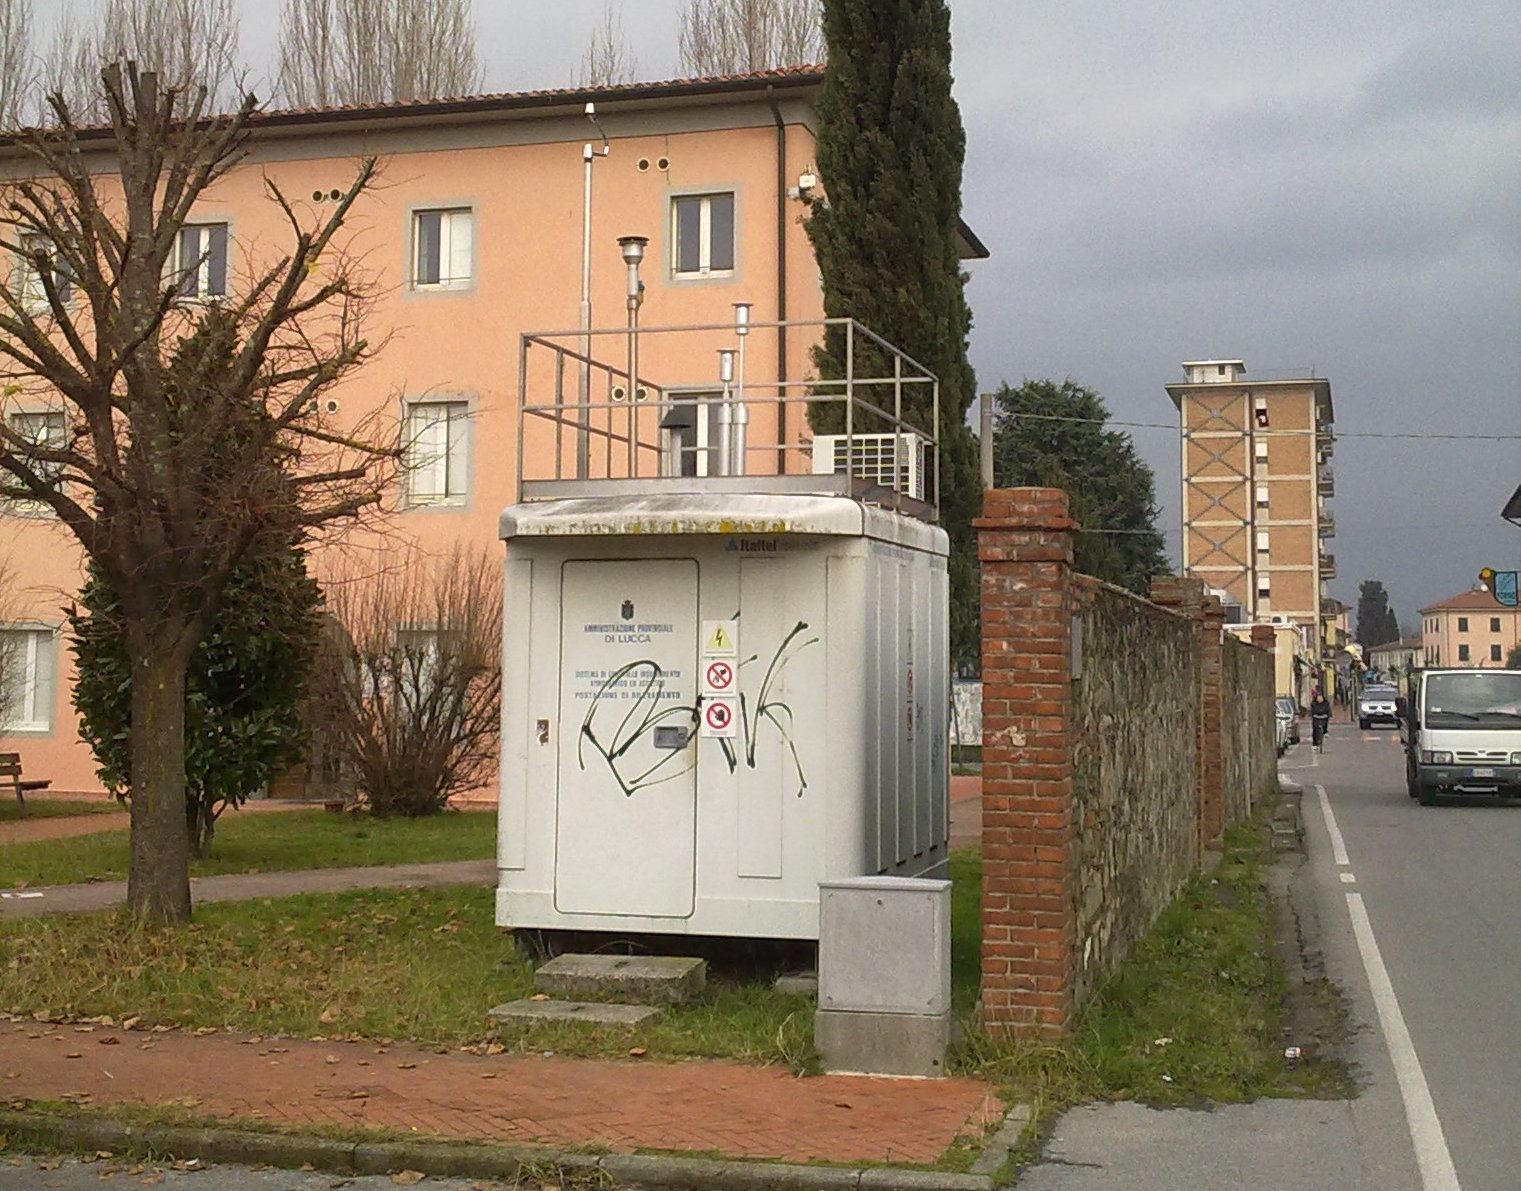
\includegraphics[width=\textwidth]{images/lu-capannori}
\caption{Stazione di rilevamento ARPAT}
\end{figure}
\end{column}

\end{columns}

\end{frame}

\begin{frame}{La piattaforma AirQino (1/3)}
\begin{columns}

\begin{column}{0.45\textwidth}

\begin{itemize}
  \item Monitoraggio ambientale ad alta precisione
  \item Configurabile ed estendibile
  \item Dati in tempo reale (PM, \ce{NO2}, \ce{CO2}, \ce{O3}, etc.)
\end{itemize}\vspace{0.1cm}

\begin{figure}[H]
\centering
\captionsetup{justification=centering}
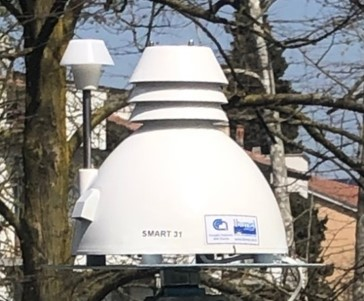
\includegraphics[width=.6\textwidth]{images/airqino_stazione}
\caption{Una centralina AirQino}
\end{figure}

\end{column}

\begin{column}{0.65\textwidth}

\begin{center}
\alert{https://airqino.magentalab.it}
\vspace{-0.3cm}
\begin{figure}[H]
\centering
\captionsetup{justification=centering}
\includegraphics[width=\textwidth]{images/airqino_web_n}
\caption{Pagina web AirQino}
\end{figure}
\end{center}

\end{column}

\end{columns}
\end{frame}

\begin{frame}[t]{La piattaforma AirQino – Architettura (2/3)}
\begin{center}

\begin{figure}[H]
\centering
\captionsetup{justification=centering}
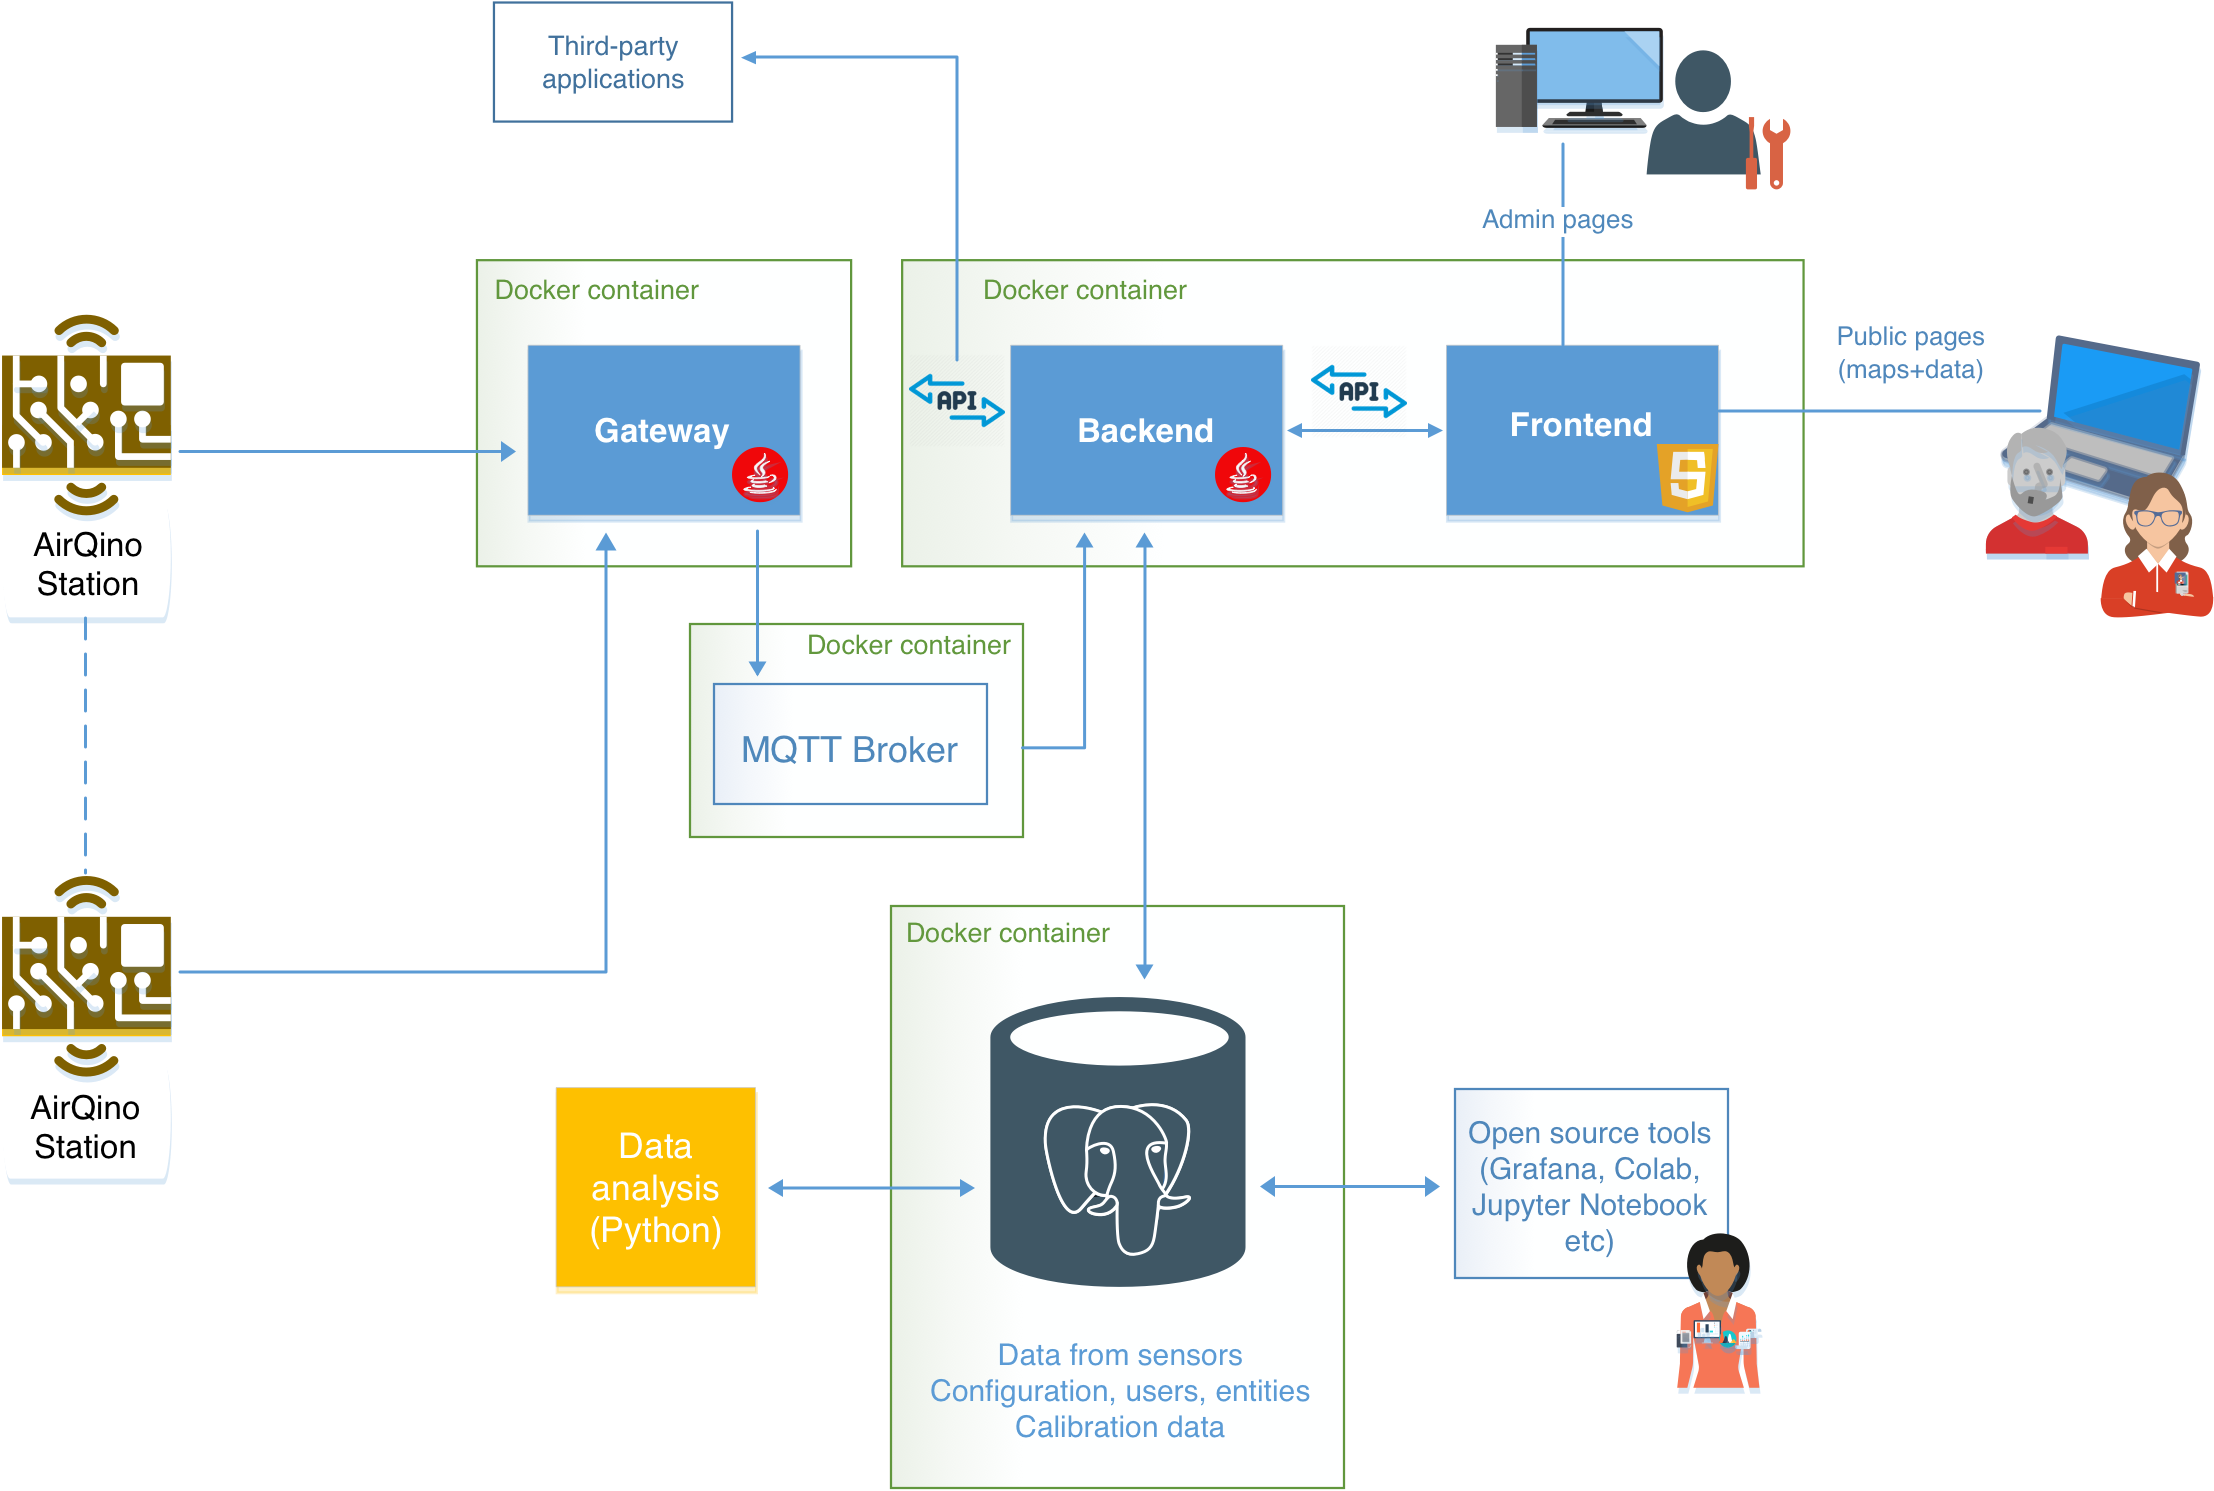
\includegraphics[width=.8\textwidth]{images/airqino_arch.png}
\caption{Architettura della piattaforma}
\end{figure}

\end{center}
\end{frame}

\begin{frame}[t]{La piattaforma AirQino – Sensori (3/3)}
\begin{columns}

\begin{column}{0.5\textwidth}
\begin{center}

\begin{block}{MiCS-2714 per \ce{NO2}}
\begin{figure}[H]
    \centering
    \subfloat[\centering Sensore]{{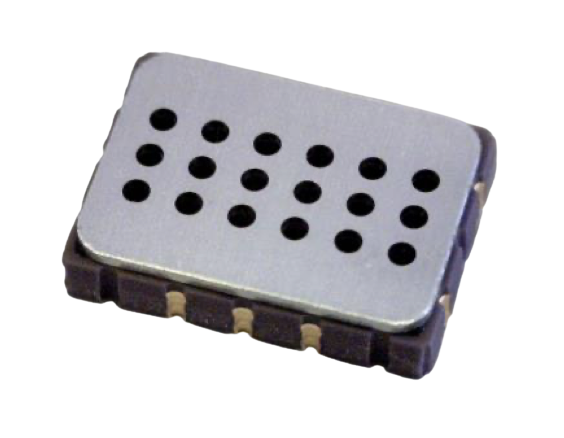
\includegraphics[width=2.4cm]{images/mics1-removebg-preview} }}
    \subfloat[\centering Circuito]{{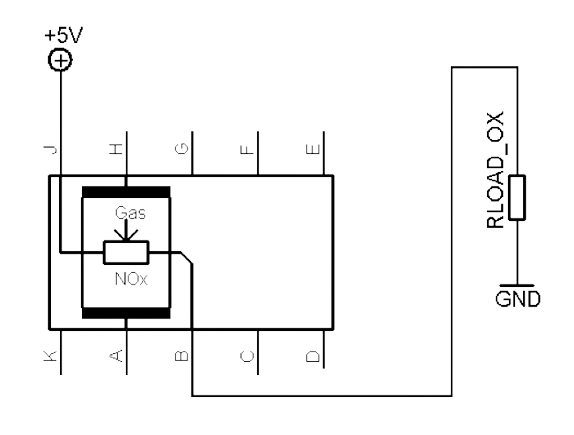
\includegraphics[width=2.4cm]{images/mics2-removebg-preview} }}
\end{figure}
\vspace{0.1cm}
\begin{itemize}
  \item Di tipo MOS, basato su \textit{ossidoriduzione}
  \item Uscita in \textit{counts}
  \item Costo: meno di 5€
\end{itemize}
\vspace{0.1cm}

\end{block}

\end{center}
\end{column}

\begin{column}{0.5\textwidth}
\begin{center}
\begin{block}{SDS011 per \ce{PM_{2.5}} e \ce{PM_{10}}}
\begin{figure}[H]
    \centering
    \subfloat[\centering Sensore]{{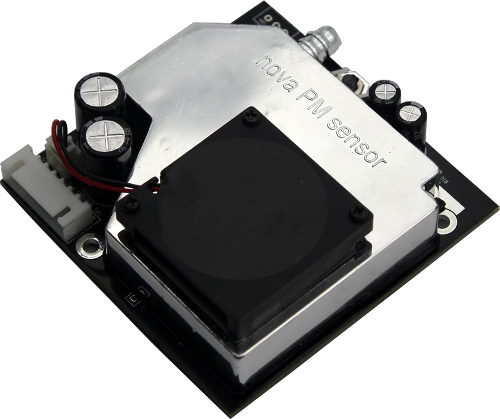
\includegraphics[width=2cm]{images/sds1} }}
    \subfloat[\centering Componenti]{{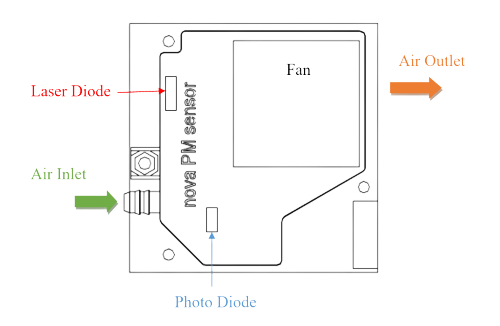
\includegraphics[width=2.7cm]{images/sds2_rmbg} }}
\end{figure}
\vspace{0.1cm}
\begin{itemize}
  \item Basato su \textit{scattering}
  \item Uscita in $\mathrm{\si{\micro}g/m^3}$
  \item Costo: 25€ circa
\end{itemize}
\vspace{0.1cm}

\end{block}
\end{center}
\end{column}

\end{columns}
\end{frame}

\begin{frame}{Attività}
\begin{itemize}
  \item Sviluppi tecnologici alla piattaforma \alert{AirQino}
  \begin{enumerate}
    \item Miglioramento dell'\textbf{affidabilità} dei dati provenienti dai sensori
    \item Riduzione dei \textbf{tempi di risposta} dal database
  \end{enumerate}\vspace{0.3cm}
  \item Studio e confronto tra diverse tecniche volte a migliorare l’accuratezza del processo di \textbf{calibrazione} dei sensori (sia \ce{NO2} che PM)\vspace{0.3cm}
  \item Sviluppo di un’\textbf{interfaccia web} per facilitare la calibrazione \textit{massiva} di centraline
\end{itemize}
\end{frame}


\section{Sviluppi tecnologici}
%\begin{frame}{Sviluppi – Replica del database (1/4)}
%\begin{block}{Replica}
%Tutti i dati presenti nel database vengono copiati e distribuiti su un altro spazio fisico. La nuova istanza agisce come nodo secondario, alleggerendo il carico dal database primario. 
%
%\vspace{0.4cm}
%\textbf{Vantaggi:}\vspace{0.1cm}
%\begin{itemize}
%  \item Maggiore \textbf{affidabilità}
%  \item Miglioramento delle \textbf{prestazioni}
%  \item Maggiore \textbf{sicurezza} dei dati
%\end{itemize}\vspace{0.1cm}
%\end{block}
%
%\end{frame}
%
%\begin{frame}{Sviluppi – Replica del database (2/4)}
%
%\begin{columns}
%
%\begin{column}{0.45\textwidth}
%\begin{block}{Streaming replication}
%Funzionalità che consente di replicare i dati in tempo reale da una istanza di database Postgres a un’altra
%
%\begin{itemize}
%  \item Replica di sola lettura
%  \item Basata su \textbf{WAL} (\textit{Write Ahead Log})
%  \item Automazione con Docker\vspace{0.1cm}
%\end{itemize}
%\end{block}
%\end{column}
%
%\begin{column}{0.55\textwidth}
%\begin{figure}[H]
%\centering
%\captionsetup{justification=centering}
%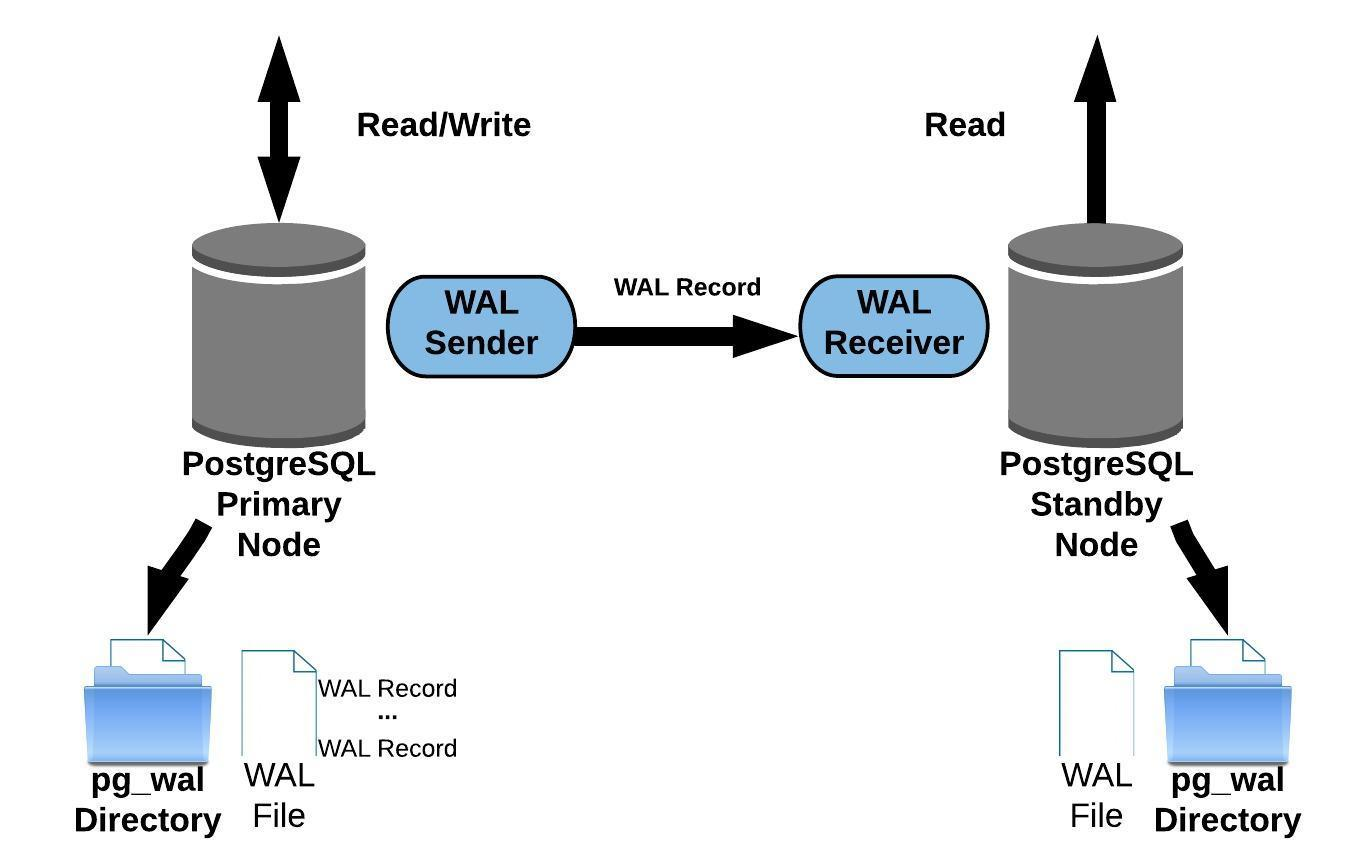
\includegraphics[width=\textwidth]{images/streaming_replication}
%\caption{Streaming replication}
%\end{figure}
%\end{column}
%
%\end{columns}
%
%\end{frame}


\begin{frame}{Sviluppi – Ottimizzazione di query temporali (1/2)}

\begin{columns}

\begin{column}{0.45\textwidth}
\begin{block}{Continuous aggregates}
Funzionalità di \textbf{Timescale} per aggregare dati in tempo reale in maniera incrementale

\begin{itemize}
  \item Miglioramento delle \textbf{performance}
  \item Aggiornamento \textbf{automatico} in background
  \item Risparmio di \textbf{spazio}\vspace{0.1cm}
\end{itemize}
\end{block}
\end{column}

\begin{column}{0.55\textwidth}
\begin{figure}[H]
\centering
\captionsetup{justification=centering}
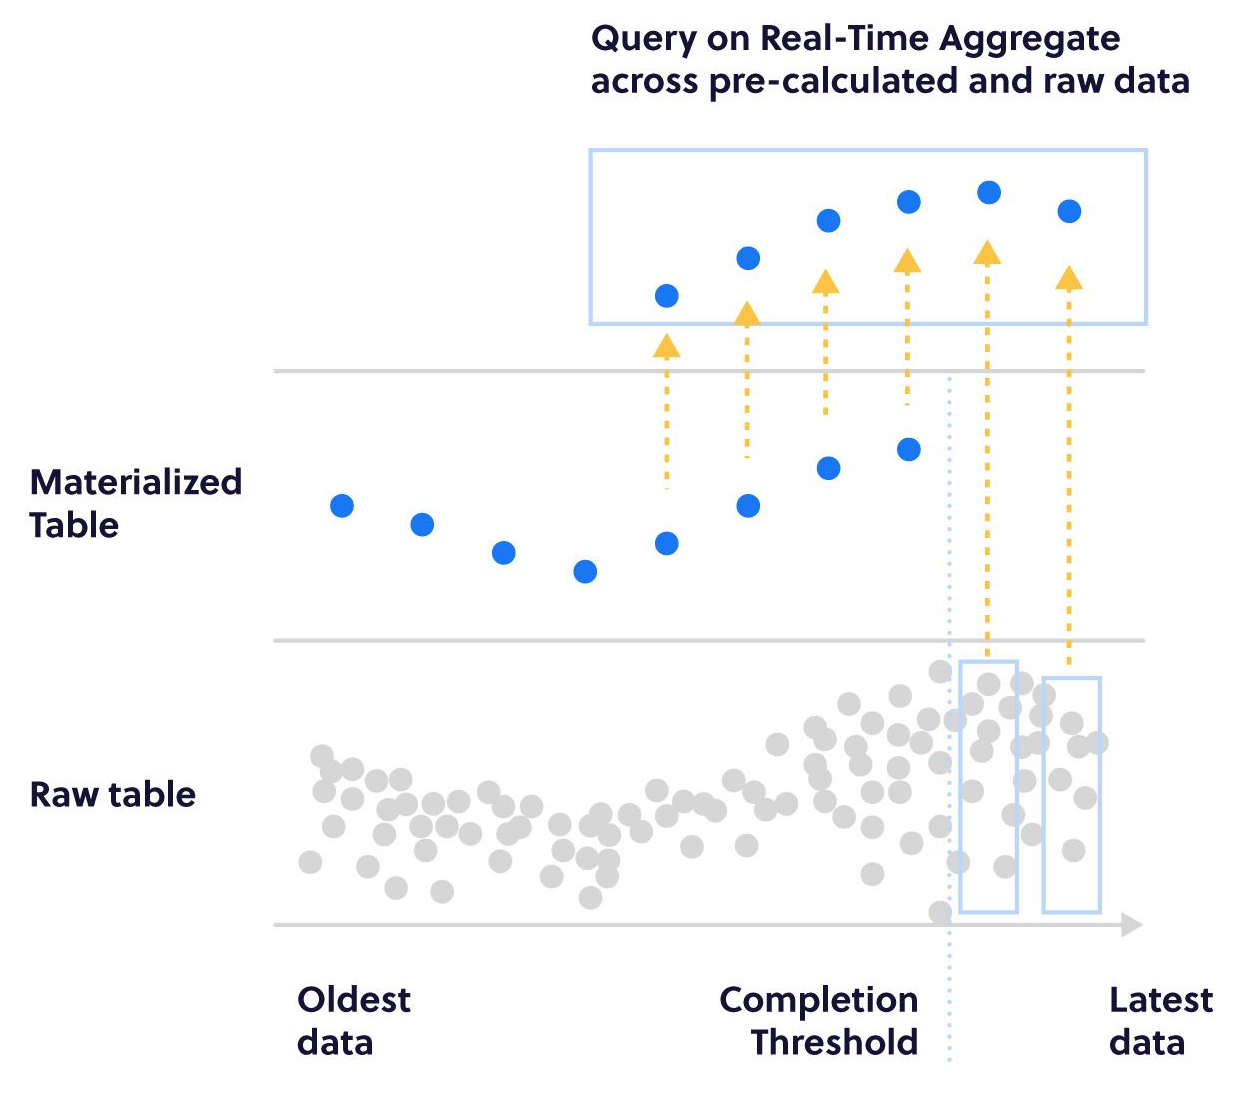
\includegraphics[width=\textwidth]{images/continuous_aggregates_r}
\caption{Continuous aggregates}
\end{figure}
\end{column}

\end{columns}

\end{frame}

\begin{frame}{Sviluppi – Ottimizzazione di query temporali (2/2)}
Tempi di risposta della query per estrarre la media oraria di \ce{NO2} dell'ultima settimana da tutte le centraline \textbf{AirQino}:

\begin{columns}
\begin{column}{0.55\textwidth}
\begin{figure}[H]
\centering
\captionsetup{justification=centering}
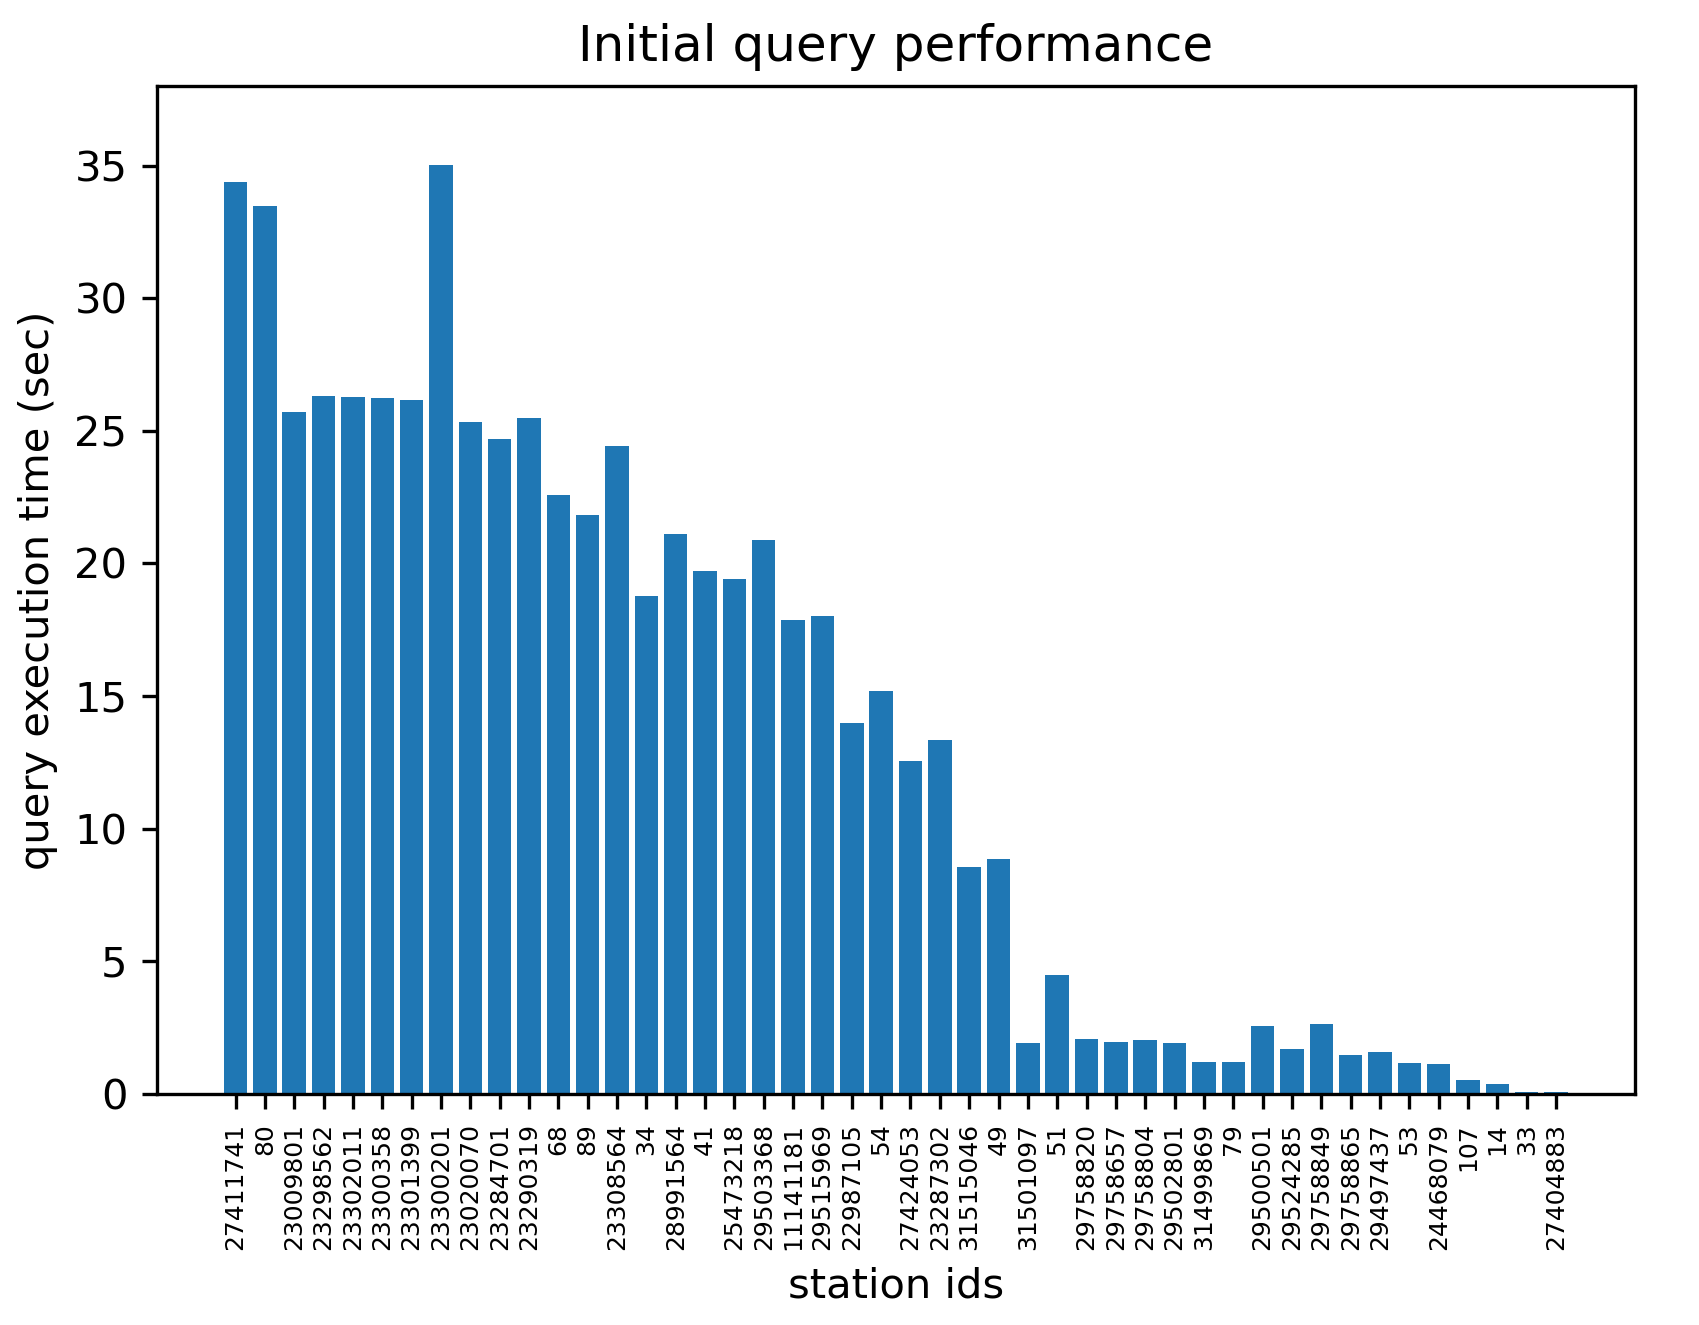
\includegraphics[width=\textwidth]{images/query_prima}
\caption{Prima dell'ottimizzazione}
\end{figure}
\end{column}

\begin{column}{0.55\textwidth}
\begin{figure}[H]
\centering
\captionsetup{justification=centering}
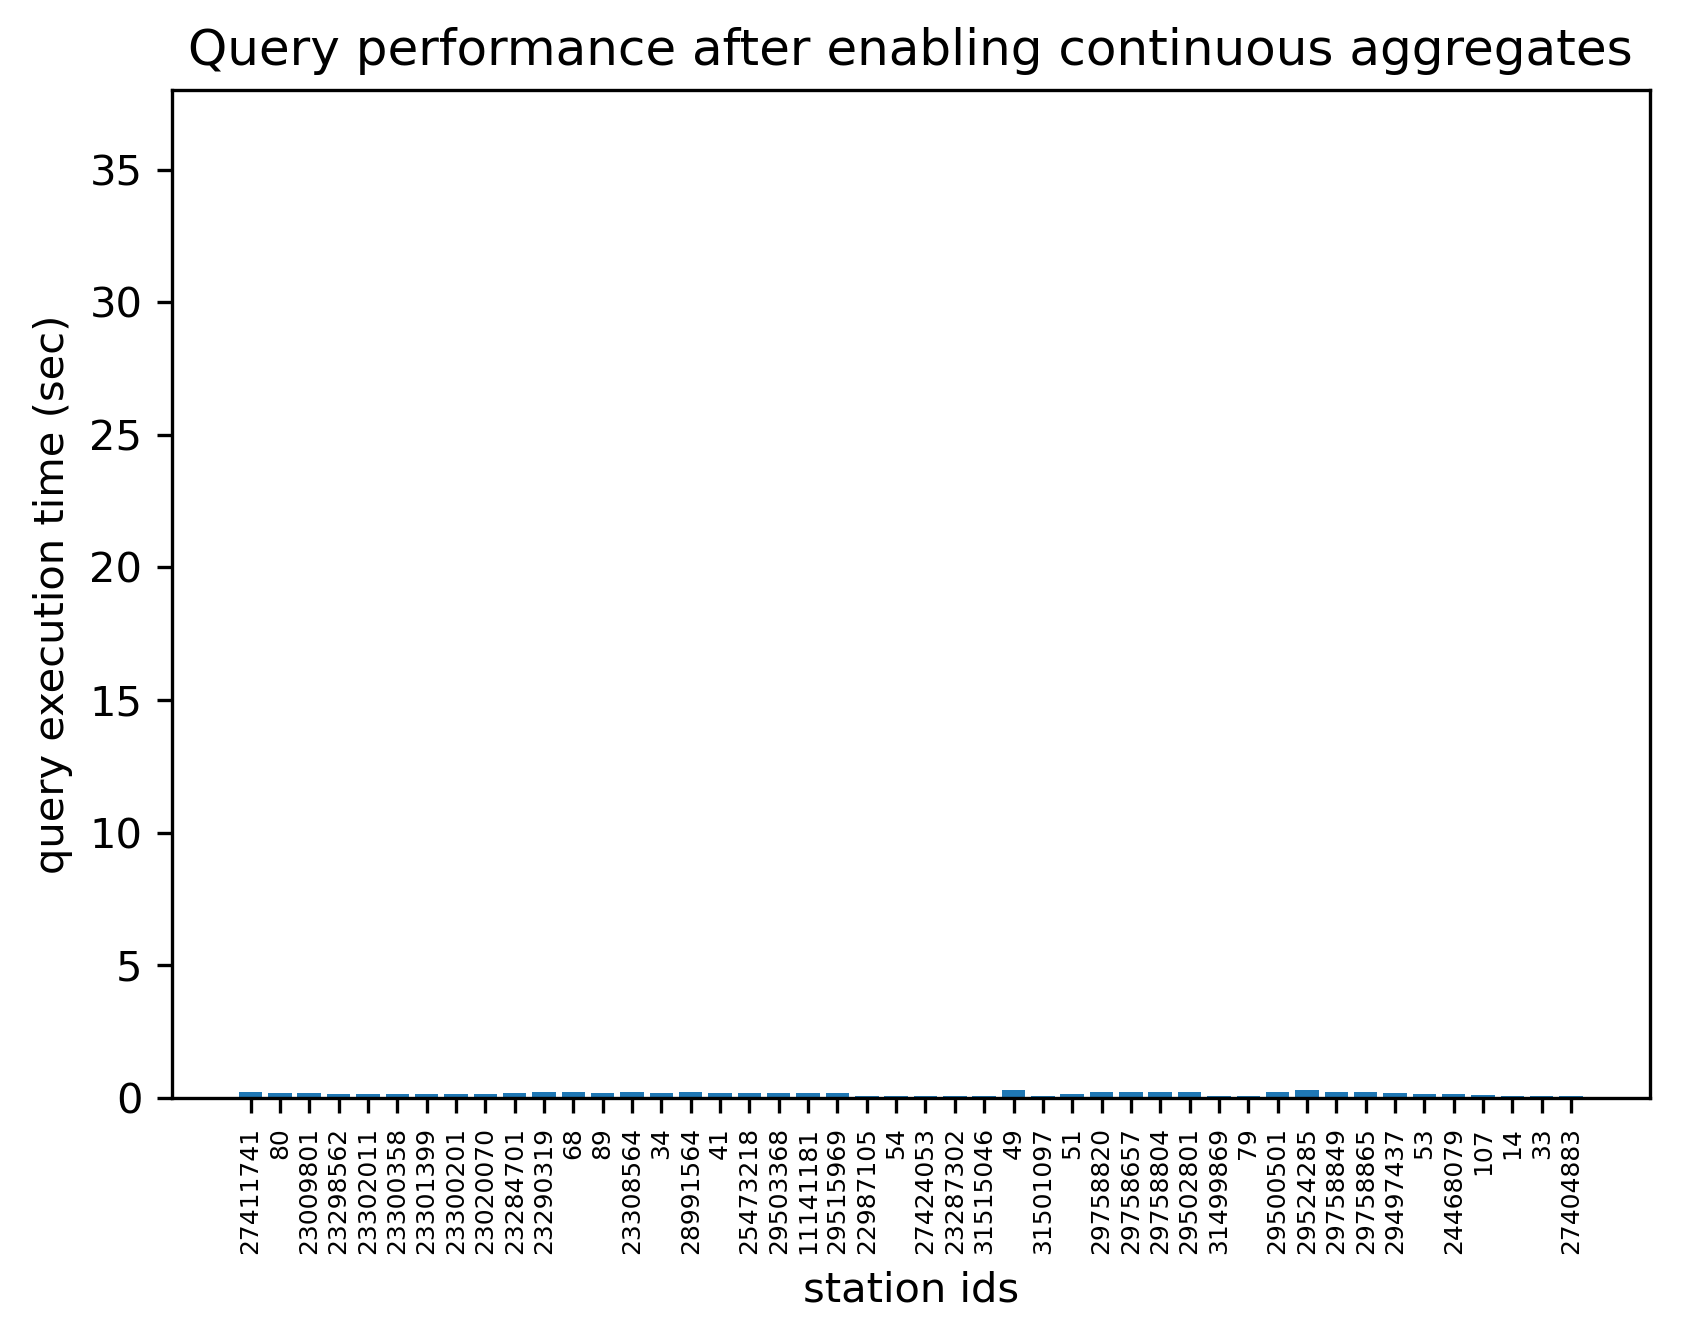
\includegraphics[width=\textwidth]{images/query_dopo}
\caption{Dopo l'ottimizzazione}
\end{figure}
\end{column}
\end{columns}

\end{frame}


\section{Calibrazione}

\begin{frame}{Calibrazione – Centraline (1/5)}
\begin{columns}
\begin{column}{0.58\textwidth}
\begin{itemize}
  \item \alert{SMART16} (AirQino), in co-locazione con la stazione \textbf{ARPAT} di Capannori (Lucca)\vspace{.1cm}
  \begin{itemize}
    \item Parte del progetto \textbf{Carilucca}\vspace{.1cm}
    \item Sito di particolare interesse data la varietà di fonti di emissione\,\footnotemark
  \end{itemize}\vspace{.05cm}
  \item \textbf{Calibrazione}: analisi della risposta dei sensori di \ce{NO2} e PM sotto diverse concentrazioni di gas (test \textit{indoor}) e comparazione verso sensori fissi di riferimento (test \textit{outdoor})
\end{itemize}
\end{column}
\begin{column}{0.46\textwidth}
\vspace{-.2cm}
\begin{center}
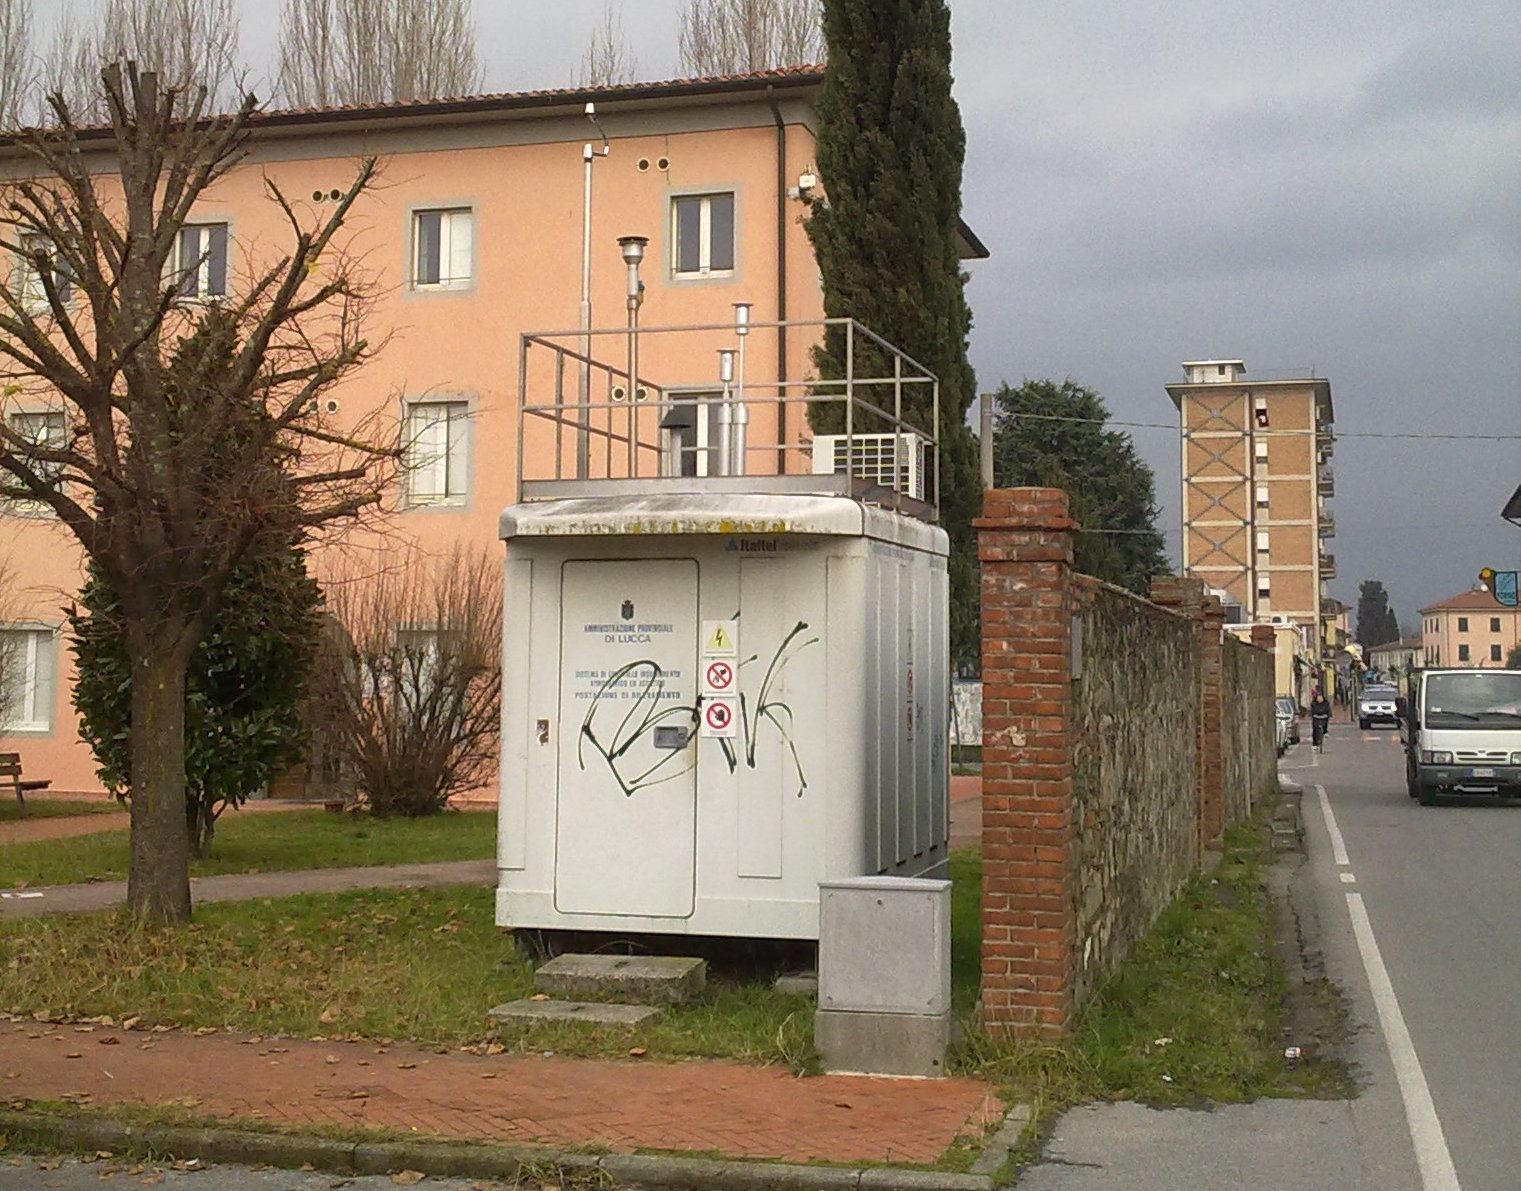
\includegraphics[width=.45\textwidth]{images/lu-capannori}
\hspace{.2cm}
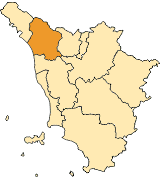
\includegraphics[width=.33\textwidth]{images/cartina-provincia-lucca}
\vspace{-.2cm}
\begin{figure}[H]
\centering
\captionsetup{justification=centering}
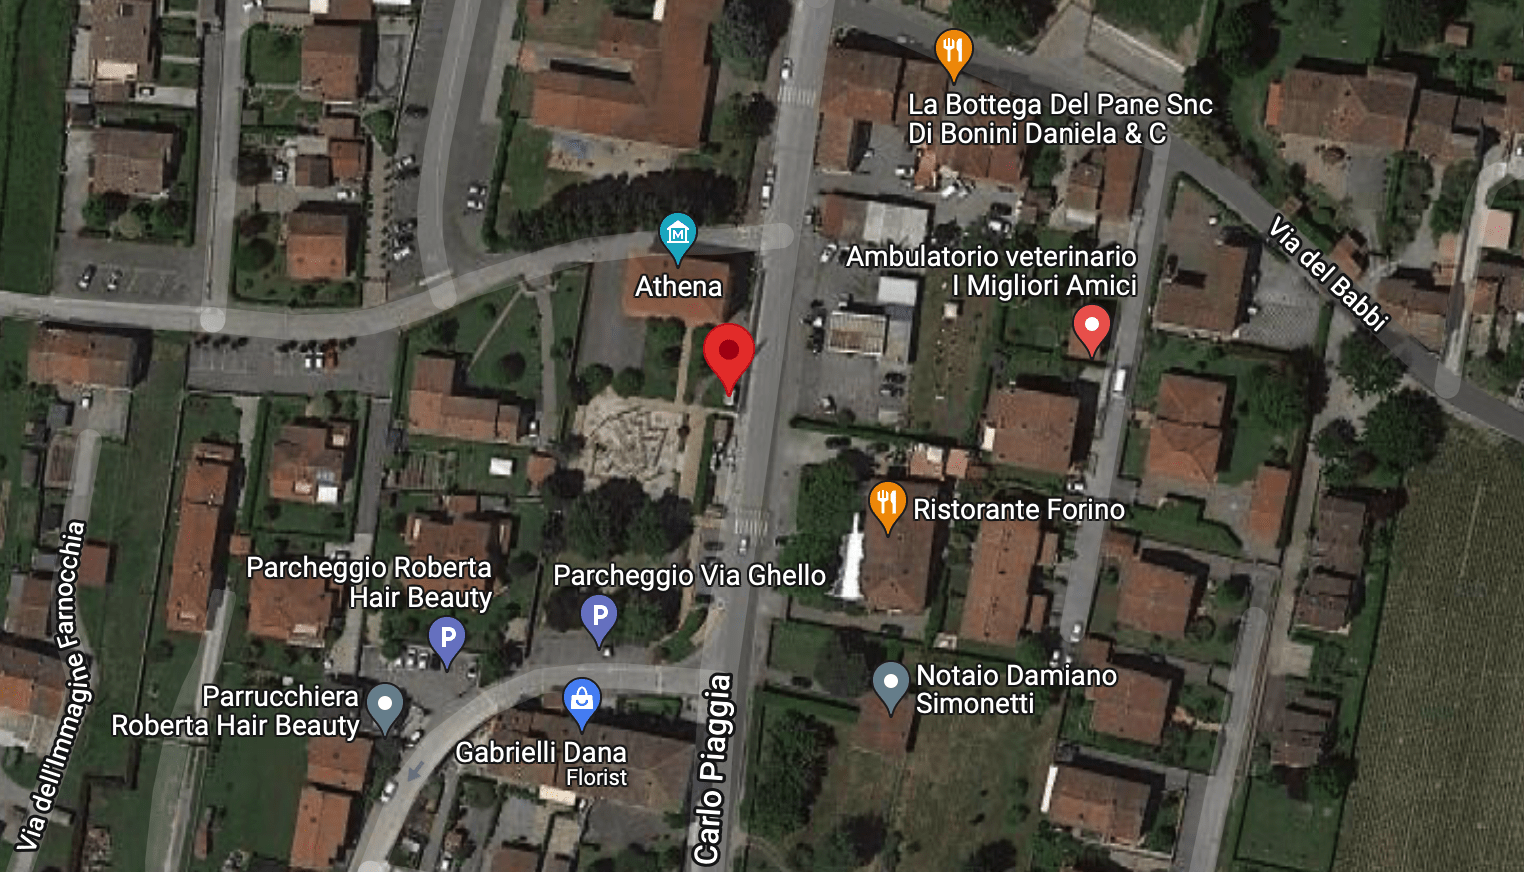
\includegraphics[width=.9\textwidth]{images/capannori_gps_r}
\caption{Posizione della centralina SMART16 (AirQino) e stazione ARPAT a Capannori (Lucca)}
\end{figure}
\end{center}
\end{column}
\end{columns}
\let\oldfootnotesize\footnotesize
\renewcommand*{\footnotesize}{\oldfootnotesize\tiny}
\addtocounter{footnote}{0}\footnotetext{\fullcite{atmos12081065}\vspace{0.05cm}}
\end{frame}

\begin{frame}{Calibrazione – Procedura (2/5)}
\begin{block}{Procedura per ogni sensore (\ce{NO2}, \ce{PM_{2.5}}, \ce{PM10})}
\begin{enumerate}
  \item Preprocessamento e creazione di un \textbf{dataset} (dati della centralina AirQino SMART16 e di riferimento ARPAT)
  \item \textbf{Allineamento} temporale e ricampionamento
  \item \textbf{Scatterplot} del segnale di riferimento e del segnale del sensore
  \item Analisi dei \textbf{residui}
  \item Applicazione di tredici diversi modelli di \alert{regressione}
  \begin{itemize}
    \item Su tutto il dataset
    \item Con cadenza mensile
  \end{itemize}
  \item Valutazione della \textbf{performance} in termini di $R^2$ e $RMSE$
  \item \textbf{Validazione} del modello più performante\vspace{0.1cm}
\end{enumerate}
\end{block}

\end{frame}

\begin{frame}{Calibrazione – Risultati (3/5)}
\begin{columns}

\begin{column}{0.55\textwidth}
\begin{center}
\textbf{Risultati \ce{NO2}} ($R^2$, $RMSE$)\vspace{0.2cm}
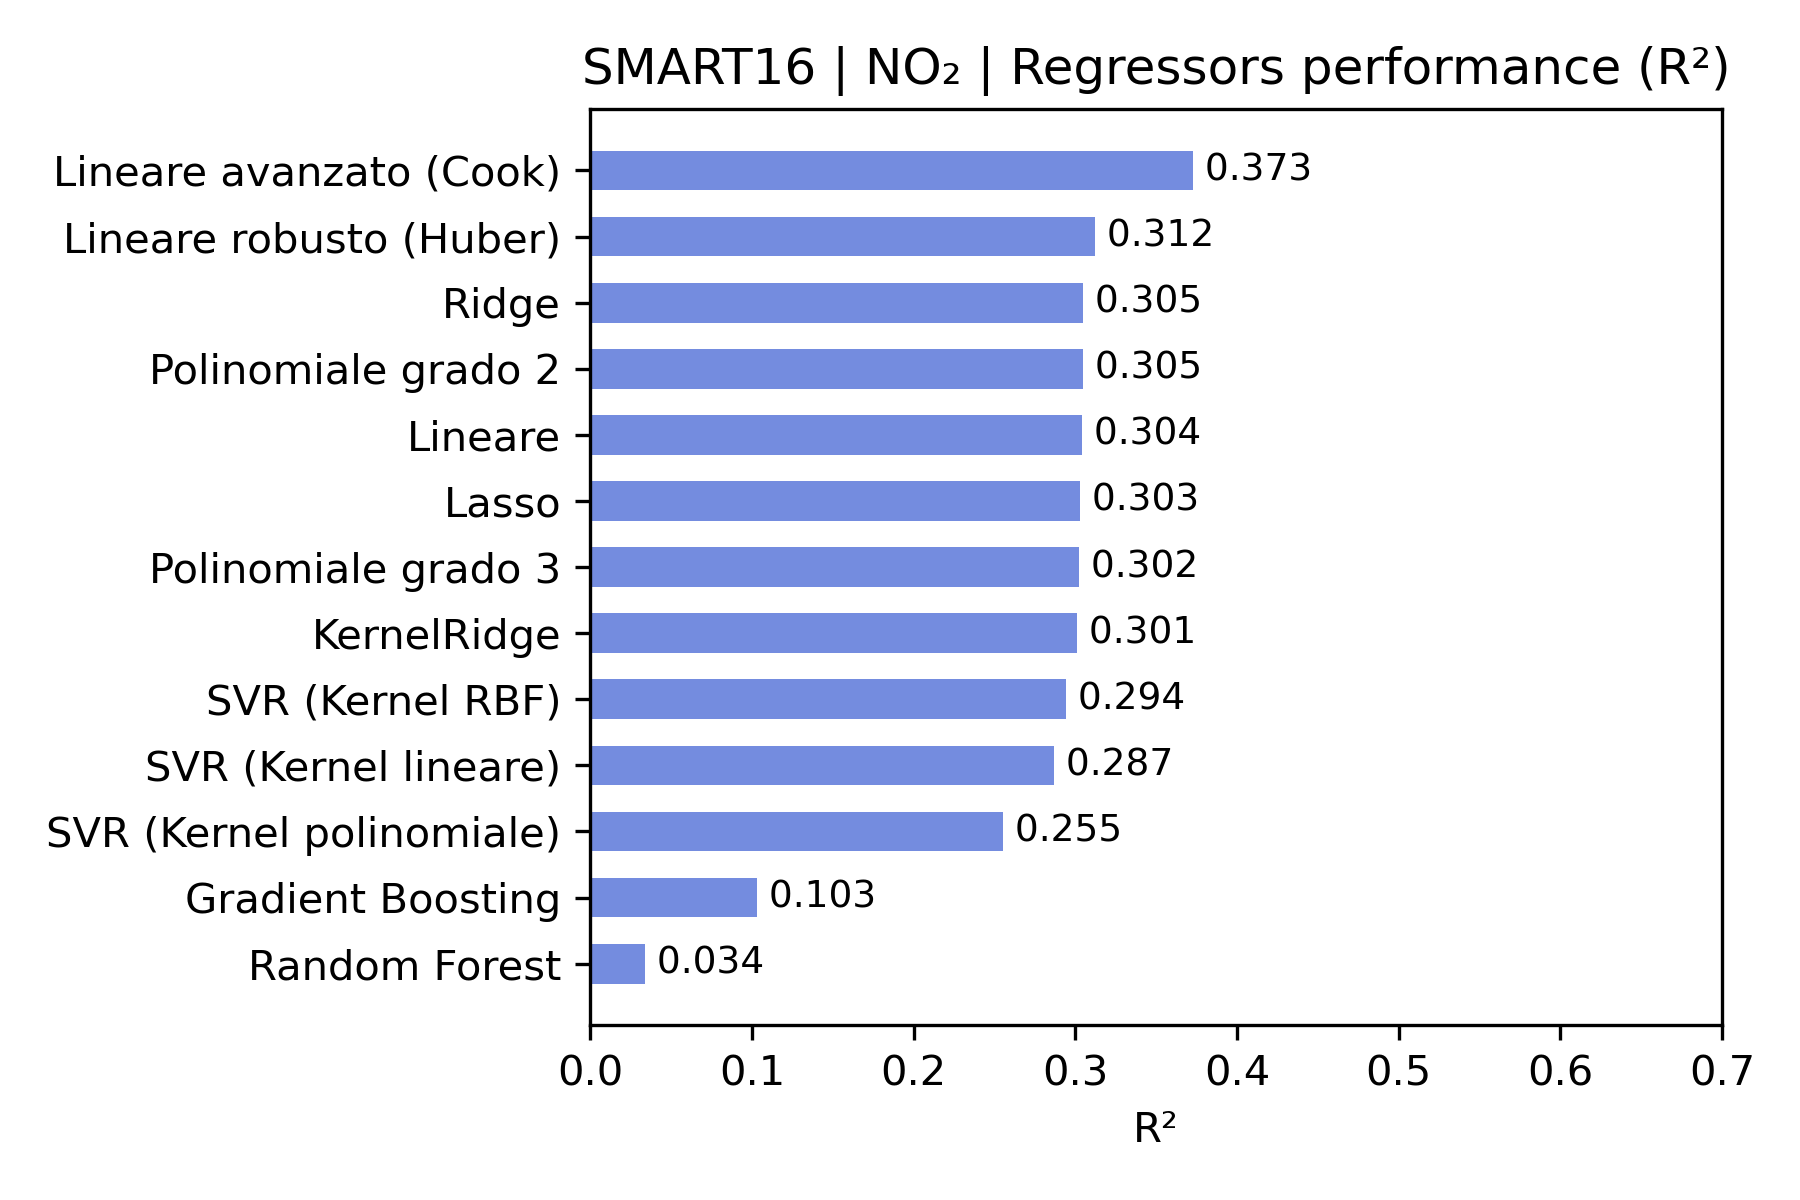
\includegraphics[width=.8\textwidth]{images/hist_no2_1}
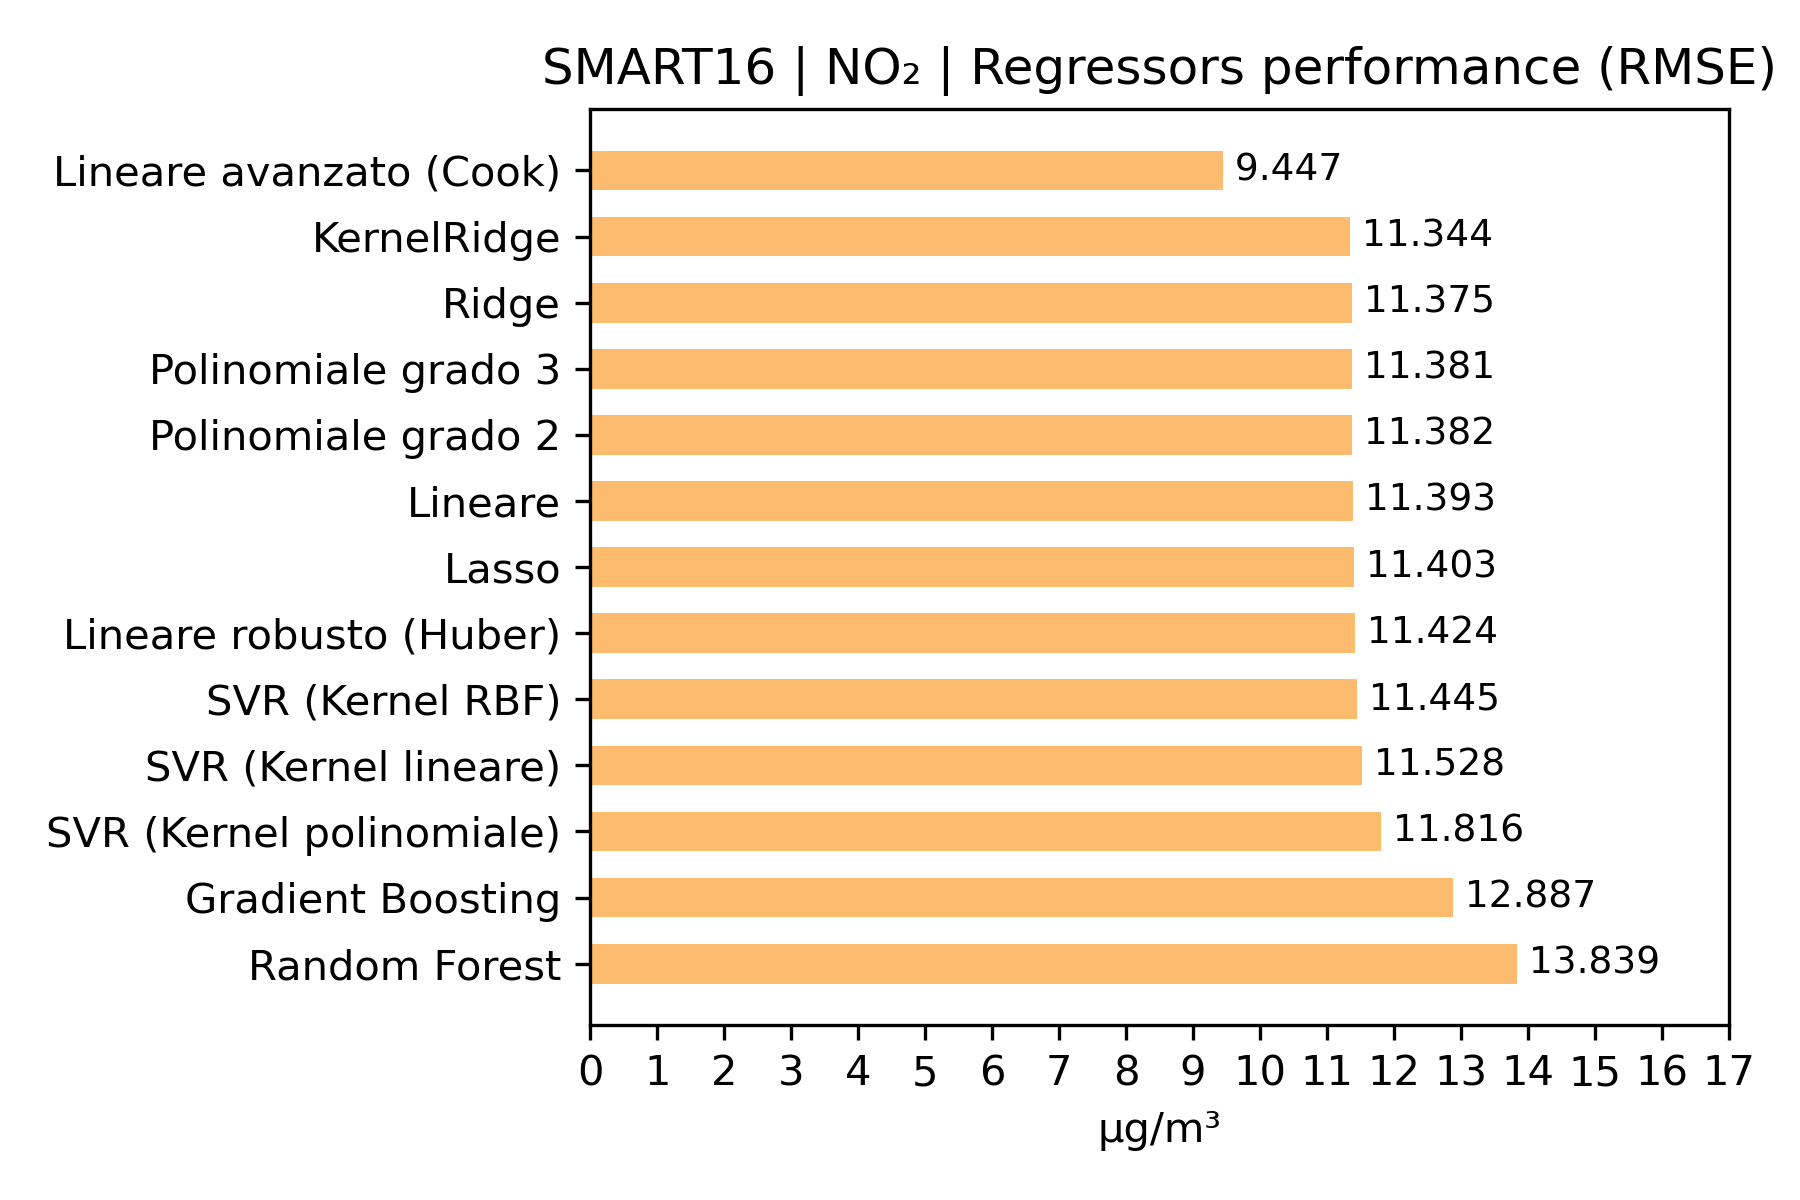
\includegraphics[width=.8\textwidth]{images/hist_no2_2}
\end{center}
\end{column}
\vrule{}
\begin{column}{0.55\textwidth}
\begin{center}
\textbf{Risultati \ce{PM_{2.5}}} ($R^2$, $RMSE$)\vspace{0.2cm}
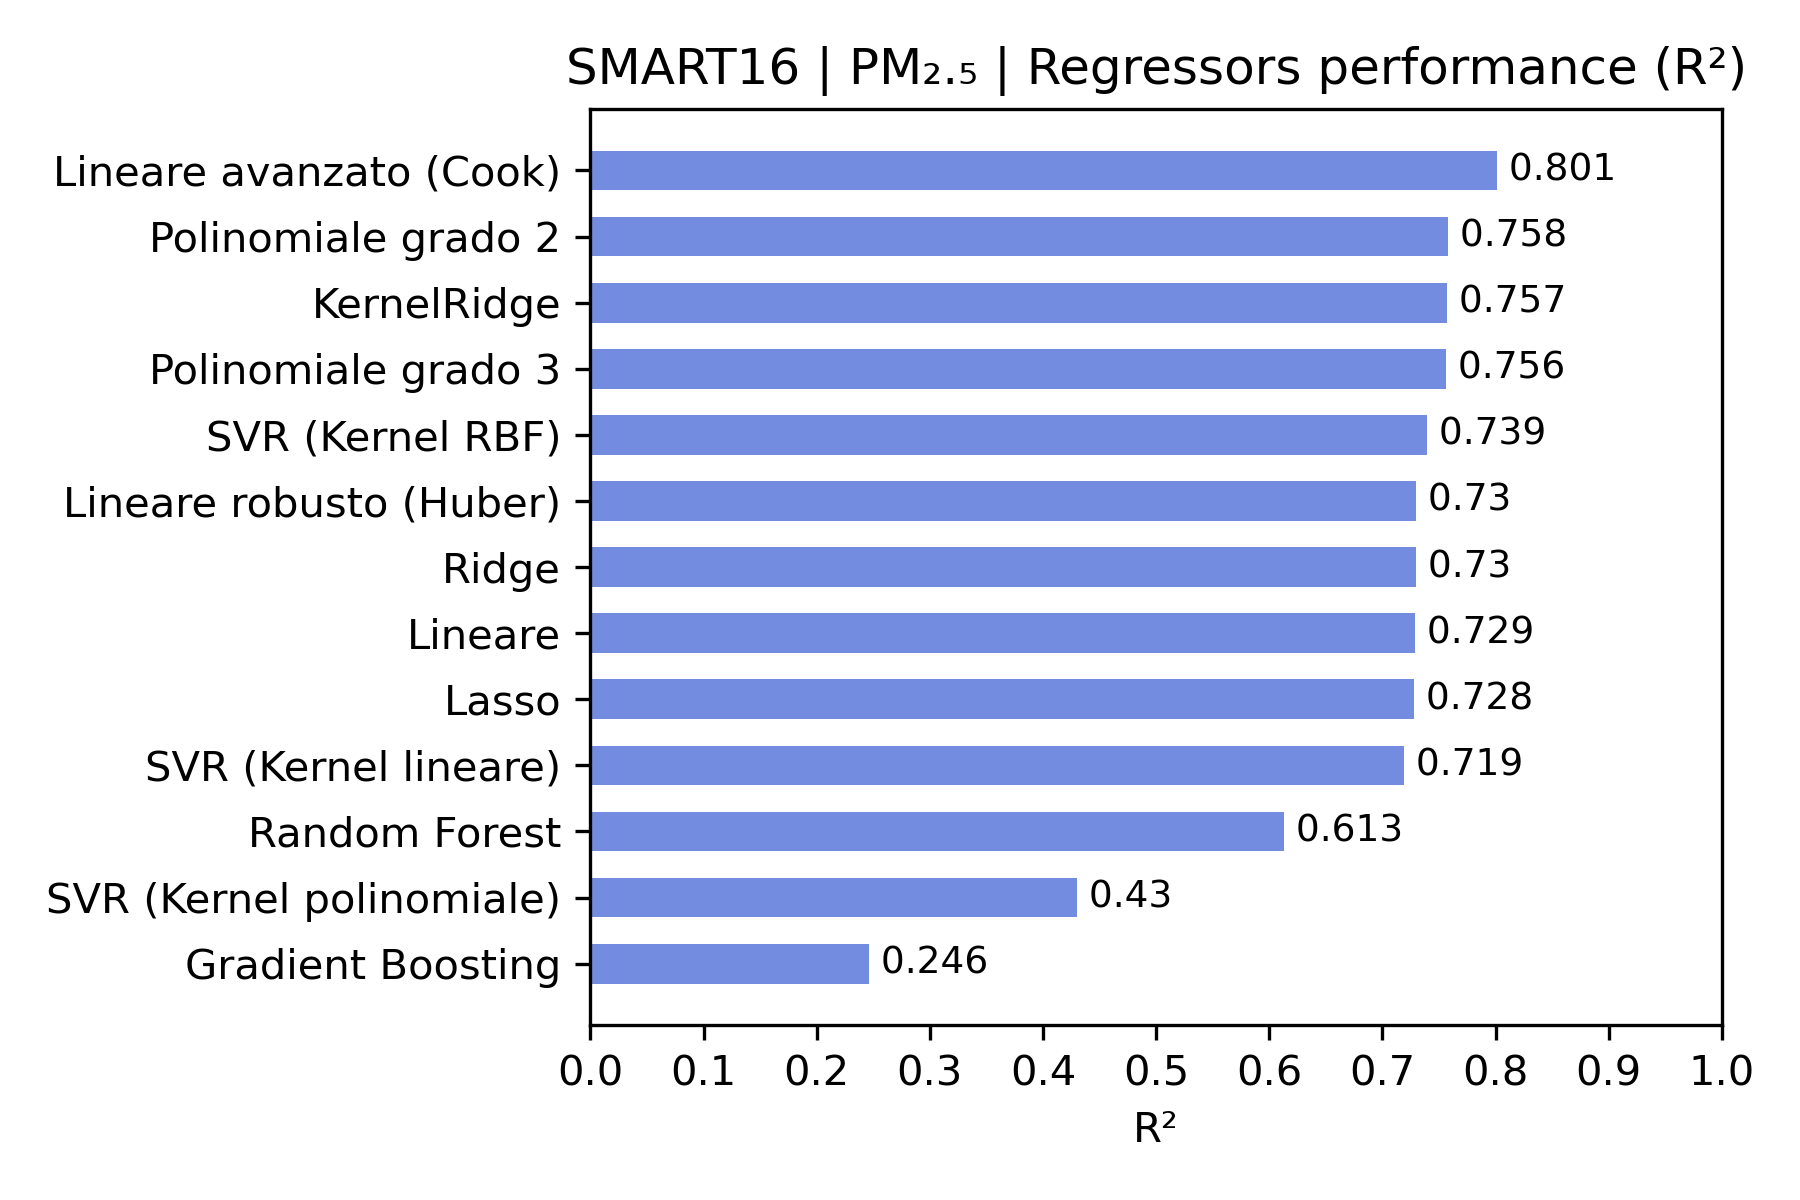
\includegraphics[width=.8\textwidth]{images/hist_pm2.5_1.png}
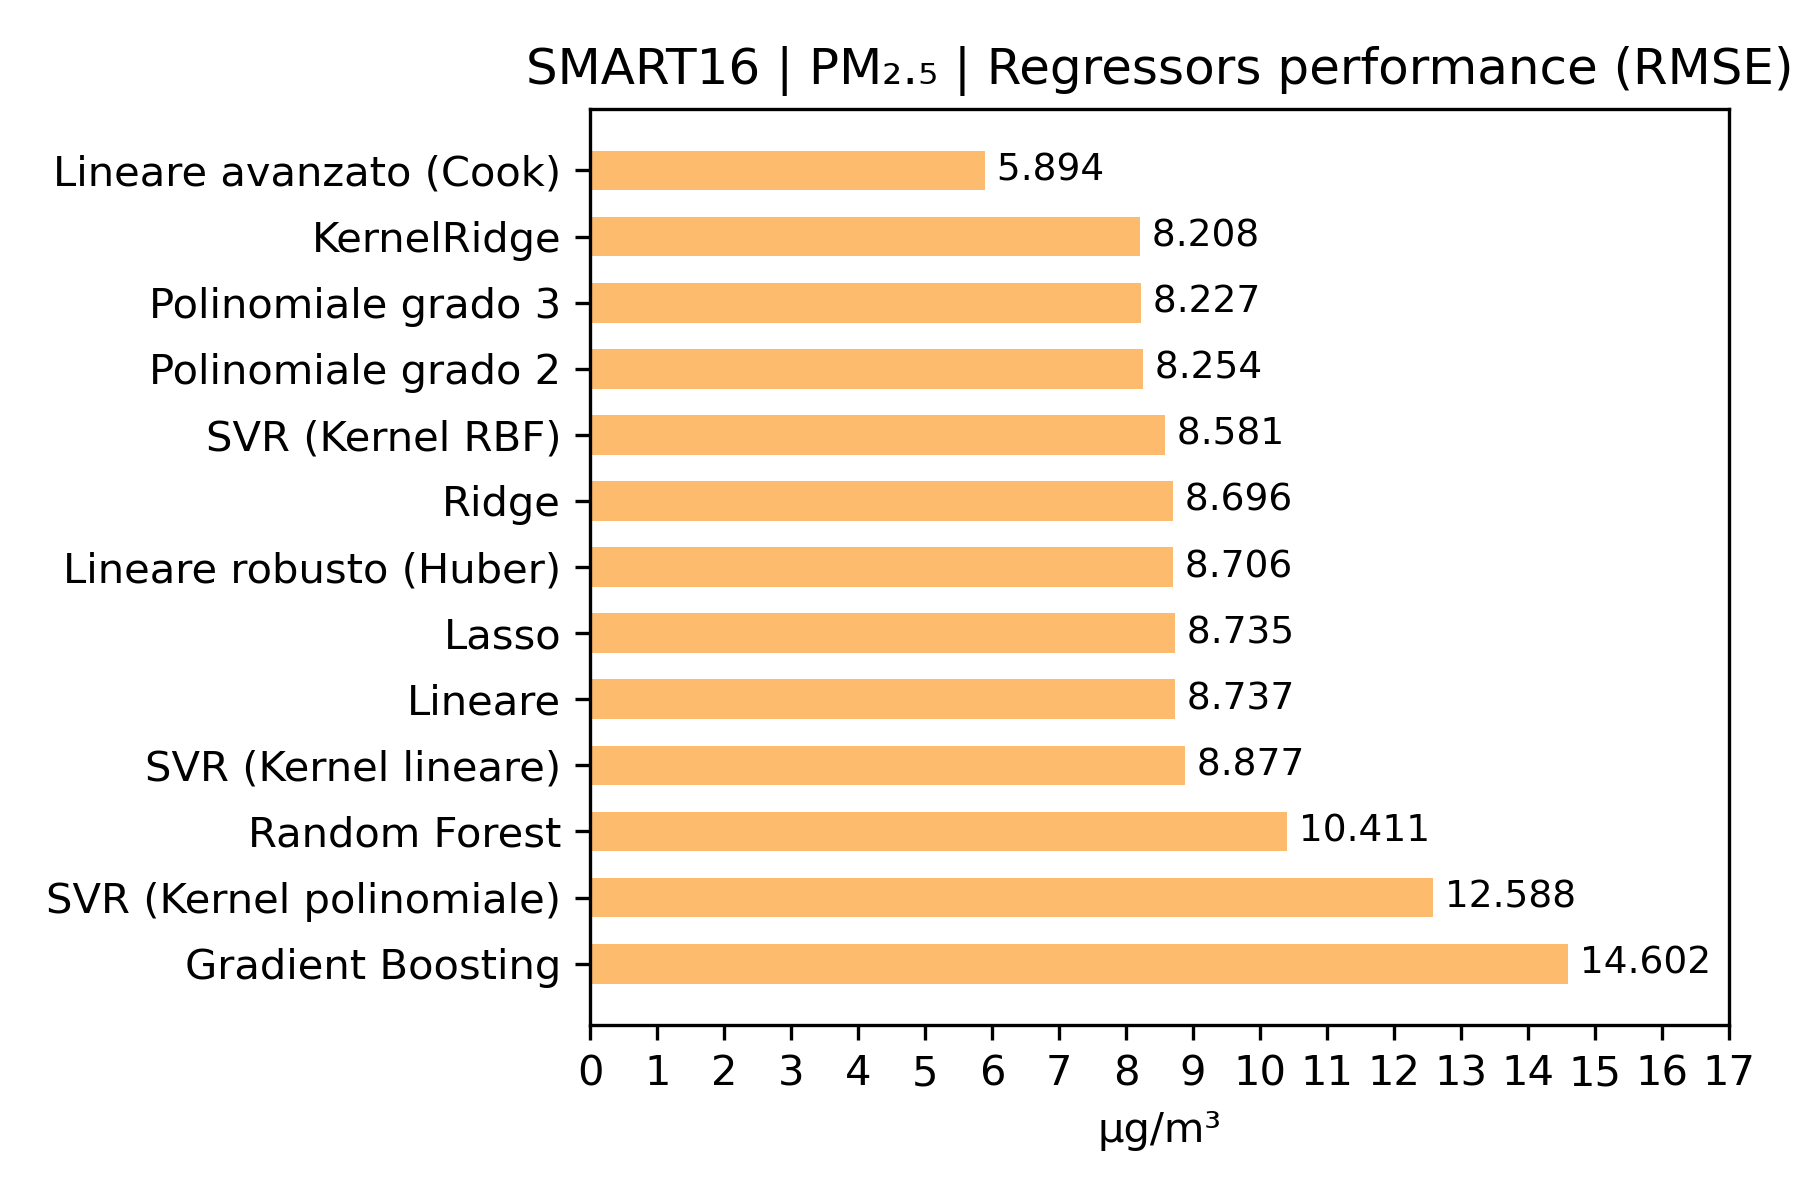
\includegraphics[width=.8\textwidth]{images/hist_pm2.5_2.png}
\end{center}
\end{column}

\end{columns}
\end{frame}

\begin{frame}{Calibrazione – Modello più performante (4/5)}

\begin{columns}
\hspace{0.3cm}\begin{column}{0.45\textwidth}

\begin{block}{Regressione lineare avanzata}
Con rimozione dei valori anomali (\textit{outlier}) in base a determinate metriche.\vspace{0.2cm}

\textbf{Distanza di Cook\,\footnotemark:}
$$D_{i}=\frac{\sum_{j=1}^{n}\left(\hat{y}_{j}-\hat{y}_{j(i)}\right)^{2}}{p  * MSE^{2}}$$

\textbf{Soglia di cut-off\,\footnotemark}:
$D_{i}>\frac{4}{n}$

\vspace{0.1cm}
\end{block}
\end{column}

\hspace{0.1cm}\begin{column}{0.53\textwidth}

\begin{center}
\begin{figure}[H]
\centering
\captionsetup{justification=centering}
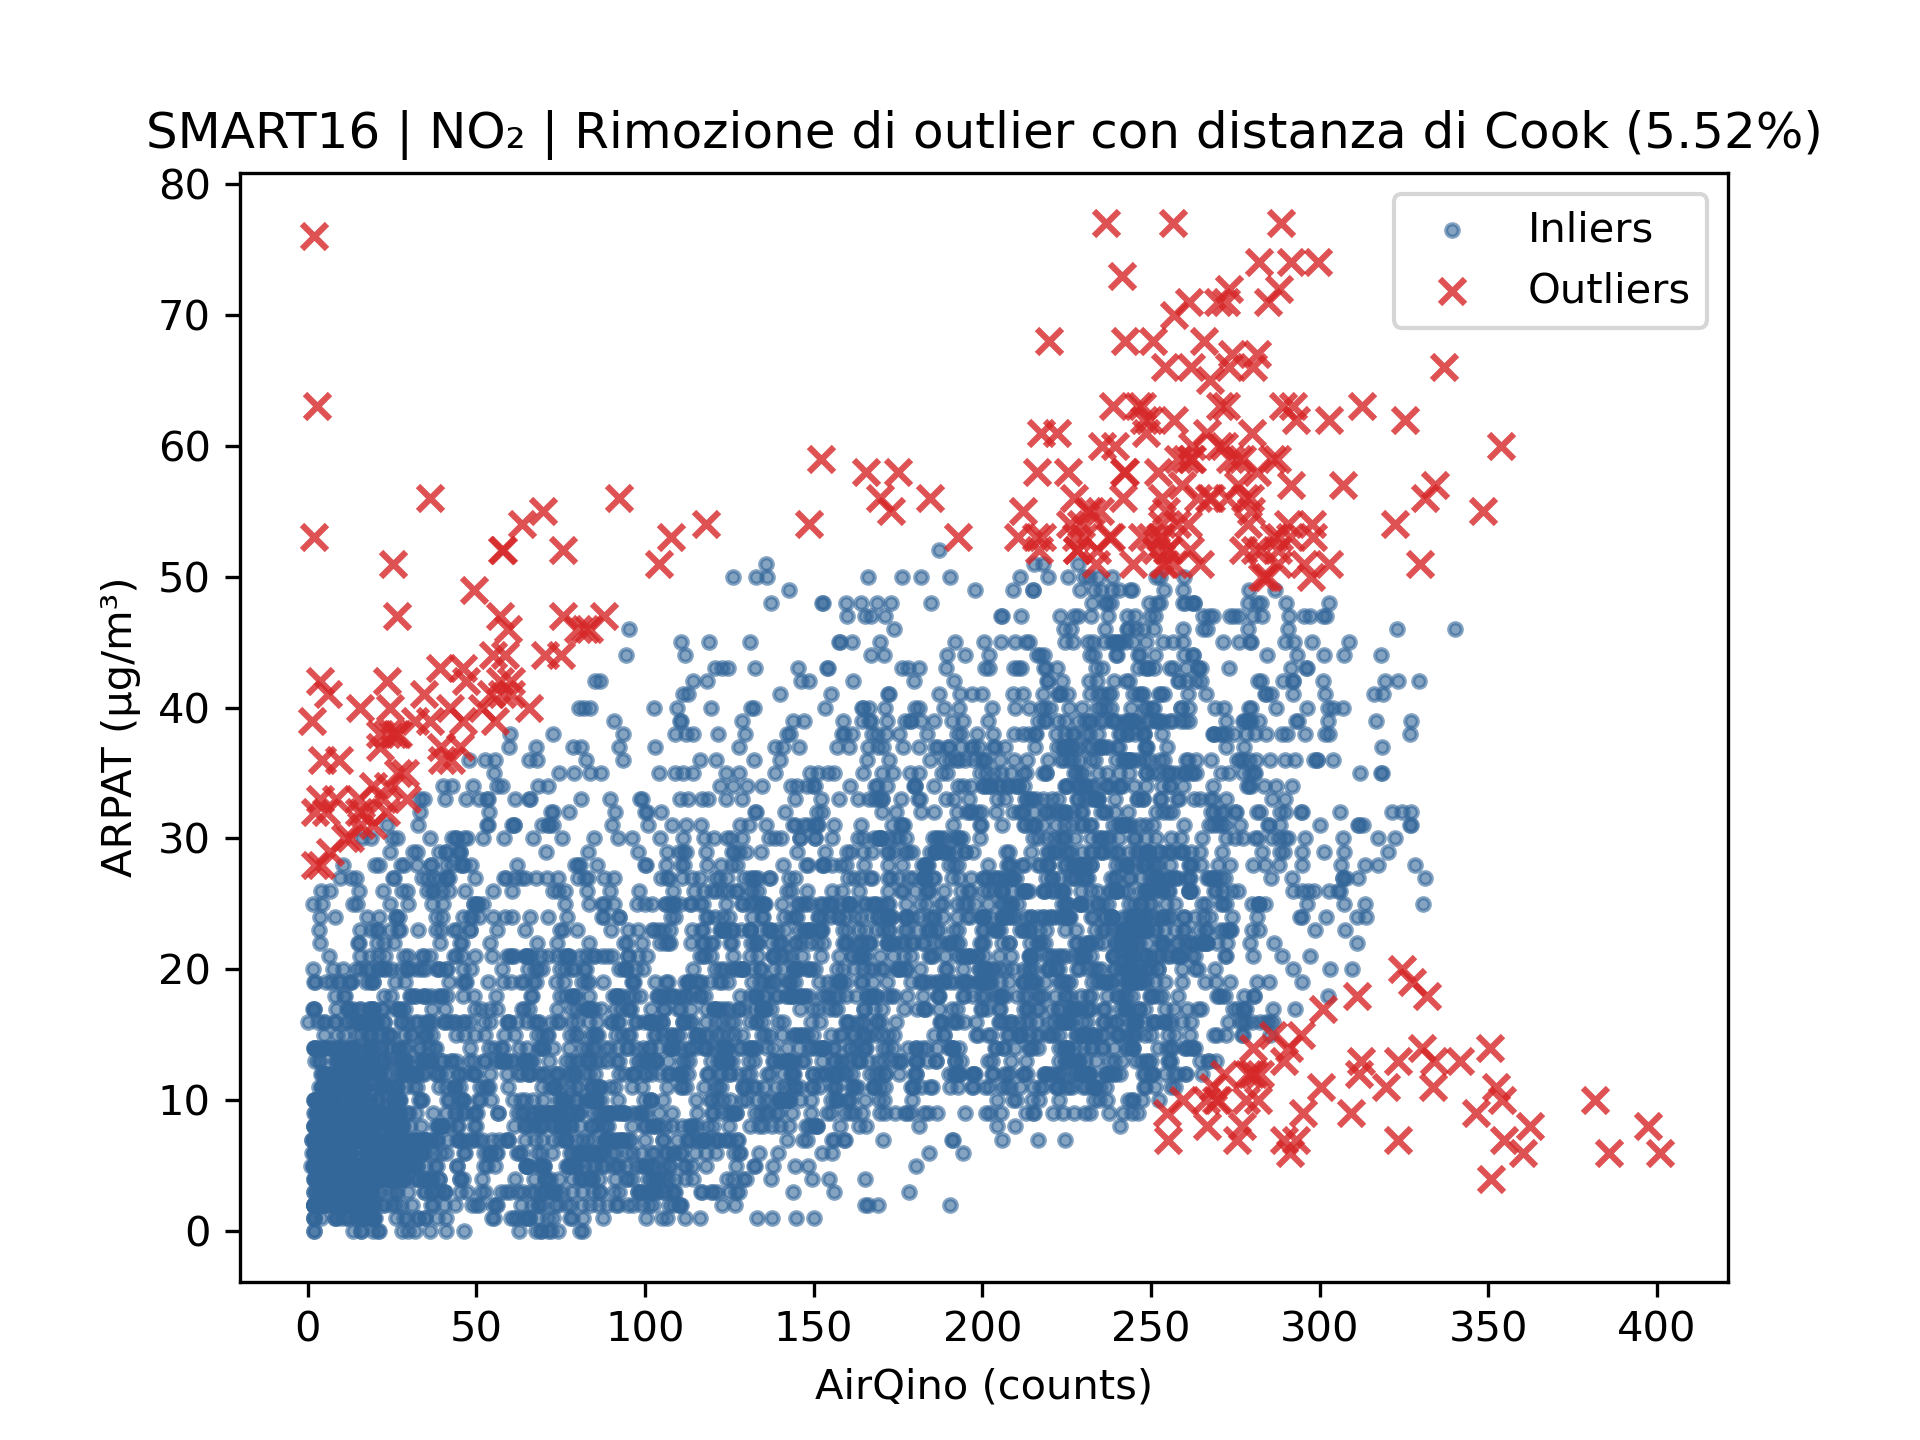
\includegraphics[width=\textwidth]{images/cook_no2.png}
\caption{Rilevamento di \textit{outlier} (in rosso) tramite distanza di Cook}
\end{figure}
\end{center}

\end{column}

\let\oldfootnotesize\footnotesize
\renewcommand*{\footnotesize}{\oldfootnotesize\tiny}
\addtocounter{footnote}{-1}\footnotetext{\fullcite{cook_def}}
\addtocounter{footnote}{1}\footnotetext{\fullcite{applied_regression}\vspace{0.05cm}}

\end{columns}

\end{frame}

\begin{frame}{Calibrazione – Validazione (5/5)}
\begin{center}
\begin{figure}[H]
\centering
\captionsetup{justification=centering}
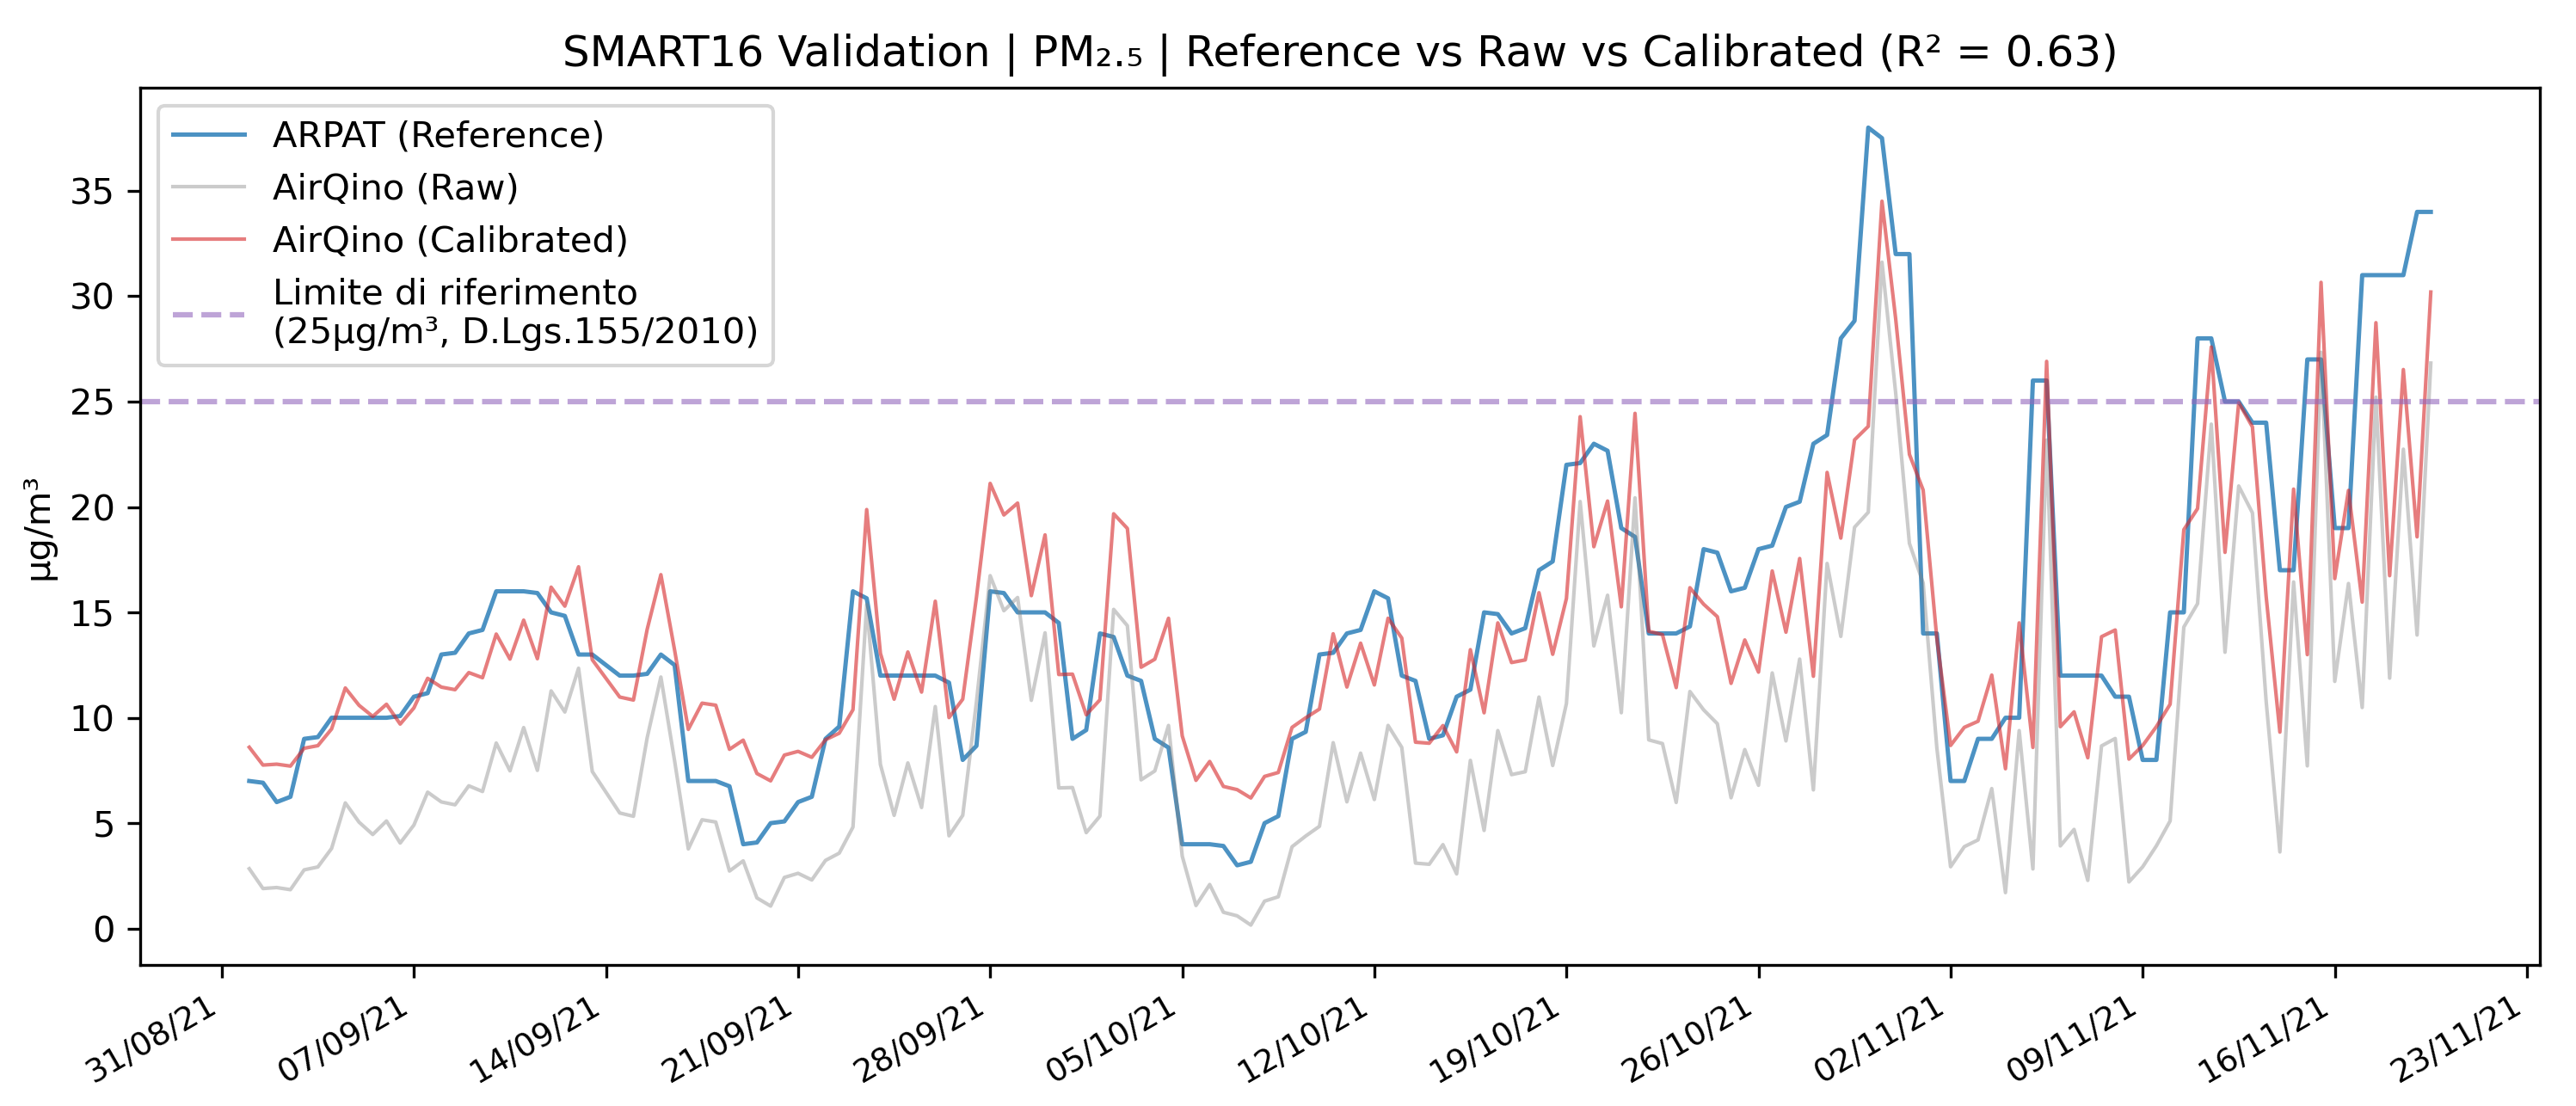
\includegraphics[width=\textwidth]{images/val_pm2.5.png}
\caption{Confronto tra l’andamento temporale delle concentrazioni di \ce{PM_{2.5}} misurate dalla stazione AirQino calibrata e non calibrata con riferimento alla stazione ARPAT di Capannori (LU). Medie a otto ore. Periodo dal 01/09/2021 al 20/11/2021.}
\end{figure}
\end{center}
\end{frame}

\section{Interfaccia}
\begin{frame}{Interfaccia utente web (1/2)}

\vspace{-0.2cm}
\begin{center}
Soluzione per la calibrazione massiva di centraline \textbf{AirQino}:  
\end{center}

\vspace{-0.2cm}
\begin{columns}

\begin{column}{0.43\textwidth}
\vspace{-.6cm}
\begin{itemize}
  \item Per permettere di inserire più \textbf{coefficienti} contemporaneamente
  \item Basata su caricamento di file \textbf{csv} appositi
  \item Con riepilogo degli esiti in forma di tabella\vspace{.1cm}
  \begin{itemize}
  \item Statistiche sui coefficienti medi
  \end{itemize}
\end{itemize}

\end{column}

\begin{column}{0.65\textwidth}

\begin{center}
\begin{figure}[H]
\centering
\captionsetup{justification=centering}
\vspace{-0.2cm}
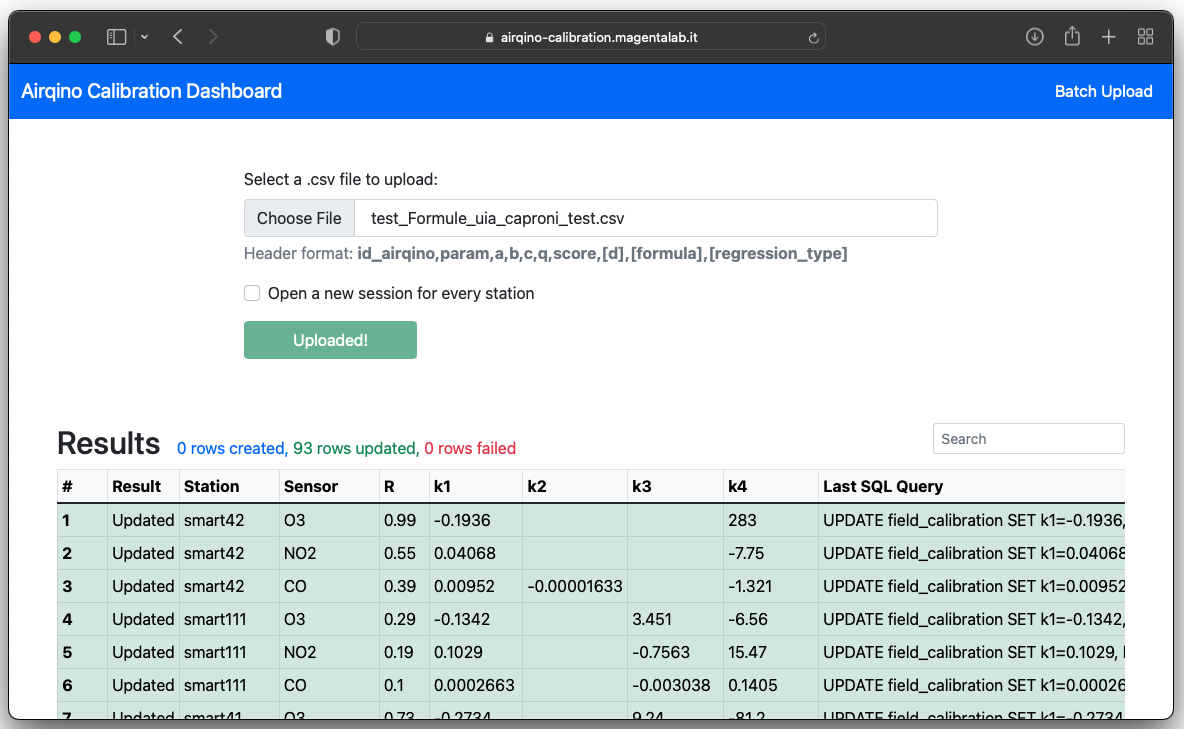
\includegraphics[width=\textwidth]{images/interfaccia_2_r}
\caption{Pagina web calibrazione}
\end{figure}
\end{center}

\end{column}

\end{columns}
\end{frame}

\begin{frame}{Interfaccia utente web (2/2)}
\begin{columns}

\begin{column}{0.43\textwidth}

\begin{itemize}
  \item Distinzione visiva per esiti diversi di ciascun sensore
  \item Con un meccanismo di \textbf{autenticazione} per proteggere da utenti di terze parti (\textit{Keycloak})
  \item Processo di rilascio automatizzato (\textit{CI/CD}) con isolamento delle dipendenze (\textit{Docker})
\end{itemize}

\end{column}

\begin{column}{0.65\textwidth}

\begin{center}
\begin{figure}[H]
\centering
\captionsetup{justification=centering}
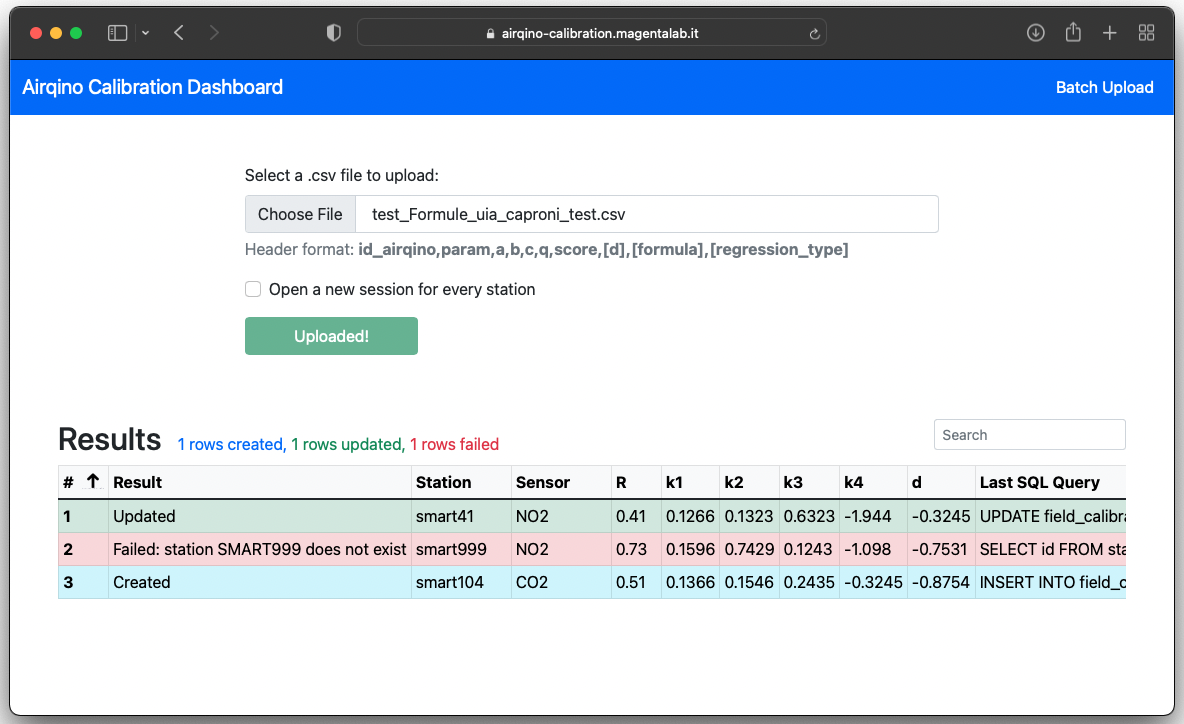
\includegraphics[width=\textwidth]{images/interfaccia_7}
\caption{Calibrazione con esiti diversi}
\end{figure}
\end{center}

\end{column}


\end{columns}
\end{frame}


\section{Conclusioni e sviluppi futuri}
\begin{frame}{Conclusioni}
\begin{itemize}
  \item Reti di sensori \textit{low-cost} per il monitoraggio della qualità dell'aria (es. \textbf{AirQino}) rappresentano una soluzione efficace per il rilevamento dell'inquinamento atmosferico\vspace{0.2cm}
  \begin{itemize}
    \item Anche in ottica di \textbf{integrazione} con le reti di monitoraggio regionali già esistenti, fornendo un quadro più completo della qualità dell'aria in ambiente urbano
  \end{itemize}\vspace{0.2cm}
  \item Anche con sensori a basso costo è possibile misurare inquinanti come \ce{NO2}, \ce{PM_{2.5}} e \ce{PM10}\vspace{0.2cm}
  \begin{itemize}
    \item Con accuratezza ancora migliore se si ha a disposizione un \textbf{segnale di riferimento} con cui correggere i dati provenienti dai sensori\vspace{0.1cm}
    \item L'applicazione di tecniche di \textbf{regressione robusta} in fase di calibrazione ha riportato miglioramenti significativi
  \end{itemize}
\end{itemize}
\end{frame}

\begin{frame}{Sviluppi futuri}
\begin{columns}

\begin{column}{0.6\textwidth}
\begin{itemize}
  \item Perfezionare il processo di calibrazione delle centraline, implementando regressioni \textit{multivariate} (includendo fattori metereologici quali \textbf{temperatura} e \textbf{umidità} relativa)\vspace{0.2cm}
  \begin{itemize}
    \item La \textbf{temperatura} tende a correlare negativamente con i PM (all'aumentare della temperatura le polveri sottili tendono a calare)\vspace{0.2cm}
    \item L'\textbf{umidità} presenta l'effetto contrario e influisce anche sull'elettronica del sensore
  \end{itemize}\vspace{0.1cm}
%  \item Realizzare una procedura di \textbf{anomaly detection} sul segnale dei sensori\vspace{0.1cm}
%  \begin{itemize}
%    \item Con un controllo \textbf{in tempo reale} sull'andamento e monitorando la differenza con il segnale di riferimento (es. stazione ARPAT)
%    \item \textbf{Post processing analysis}
%  \end{itemize}
\end{itemize}

\end{column}

\begin{column}{0.45\textwidth}
\begin{figure}[H]
\centering
\captionsetup{justification=centering}
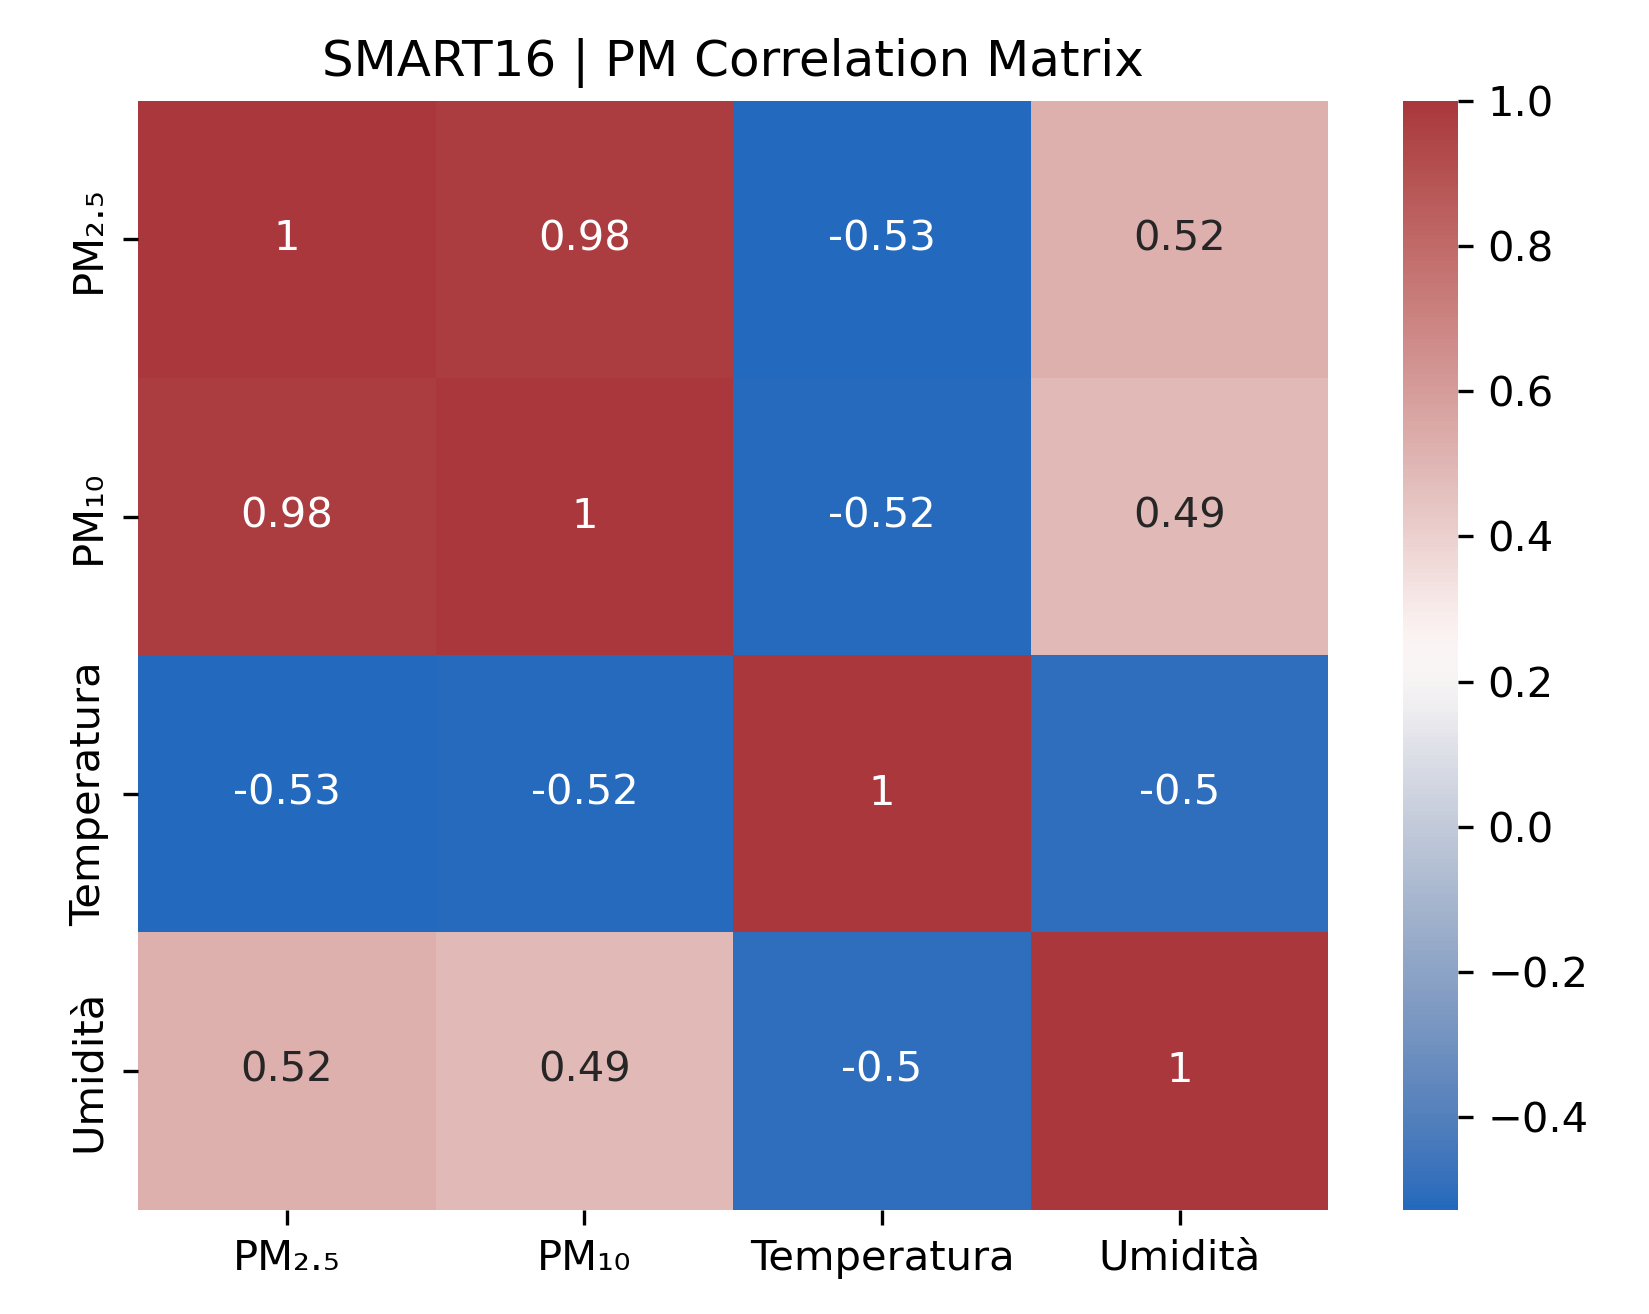
\includegraphics[width=\textwidth]{images/corr}
\caption{Correlazione tra polveri sottili, temperatura e umidità misurate dalla centralina SMART16 (periodo dal 18/08/2020 al 30/08/2021)}
\end{figure}
\end{column}

\end{columns}
\end{frame}

\begin{frame}[noframenumbering]{Grazie per l'attenzione!}
\begin{columns}

\begin{column}{0.79\textwidth}
\begin{center}
\includegraphics[width=\textwidth]{images/airqino_web_n}
\end{center}
\end{column}

\begin{column}{0.25\textwidth}\vspace{-.1cm}
\begin{center}

\includegraphics[width=\textwidth]{images/airqino}\vspace{0.4cm}

\includegraphics[width=\textwidth]{images/magenta}\vspace{0.5cm}

\includegraphics[width=\textwidth]{images/ibe}
\end{center}
\end{column}

\end{columns}

\end{frame}

